\documentclass[french, a4paper, 12pt]{report}
\usepackage[margin=2.5cm]{geometry}
\usepackage[utf8]{inputenc}
\usepackage[frenchb]{babel}
\usepackage[T1]{fontenc}
\usepackage{babel}
\usepackage{graphicx}
\usepackage{lettrine}
\usepackage{lmodern}
\usepackage{eso-pic}
\usepackage{tabularx}
\usepackage{titlesec}
\usepackage{colortbl}
\usepackage{xcolor}
\usepackage{setspace}
\usepackage{tikz}
\usepackage{hyperref}
\usepackage{stmaryrd}
\usepackage{subfig}
\usepackage{graphicx} 
\usepackage{caption}
\usepackage{mwe}
\usepackage{lipsum}
\usepackage{filecontents}
\usepackage{wrapfig}
\usepackage{url}
\usepackage{pdfpages}
\hypersetup{
    colorlinks=true,
%     linkcolor=blue,
    citecolor=black,
    filecolor=black,
    linkcolor=black,
    urlcolor=black
}


\definecolor{olivegreen}{rgb}{0,0.5,0}

\titleformat{\chapter}[hang]{\bf\LARGE}{\thechapter}{0pc}{ - }
\titleformat{\section}[hang]{\bf\Large}{\thesection}{0pc}{ - }
\titleformat{name=\chapter,numberless}[hang]{\bf\LARGE}{}{0pc}{}
\titleformat{name=\section,numberless}[hang]{\bf\Large}{\thesection}{0pc}{}
%%%%%%%%%%%%%%%%%%%%%%%%%%%%%%%%%%%%%%%%%%%%%%%%%%%%%
%%%%%%%%%%%%% PROJECT TITLE%%%%%%%%%%%%%%%%%%%%%%%%%

\title{Mémoire fin d'étude }


%%%%%%%%%%%%%%%%%%%%%%%%%%%%%%%%%%%%%%%%%%%%%%%%%%%%




\begin{document}
%%%%%%%%%%%%%%%%%%
%%% First page %%%
%%%%%%%%%%%%%%%%%%
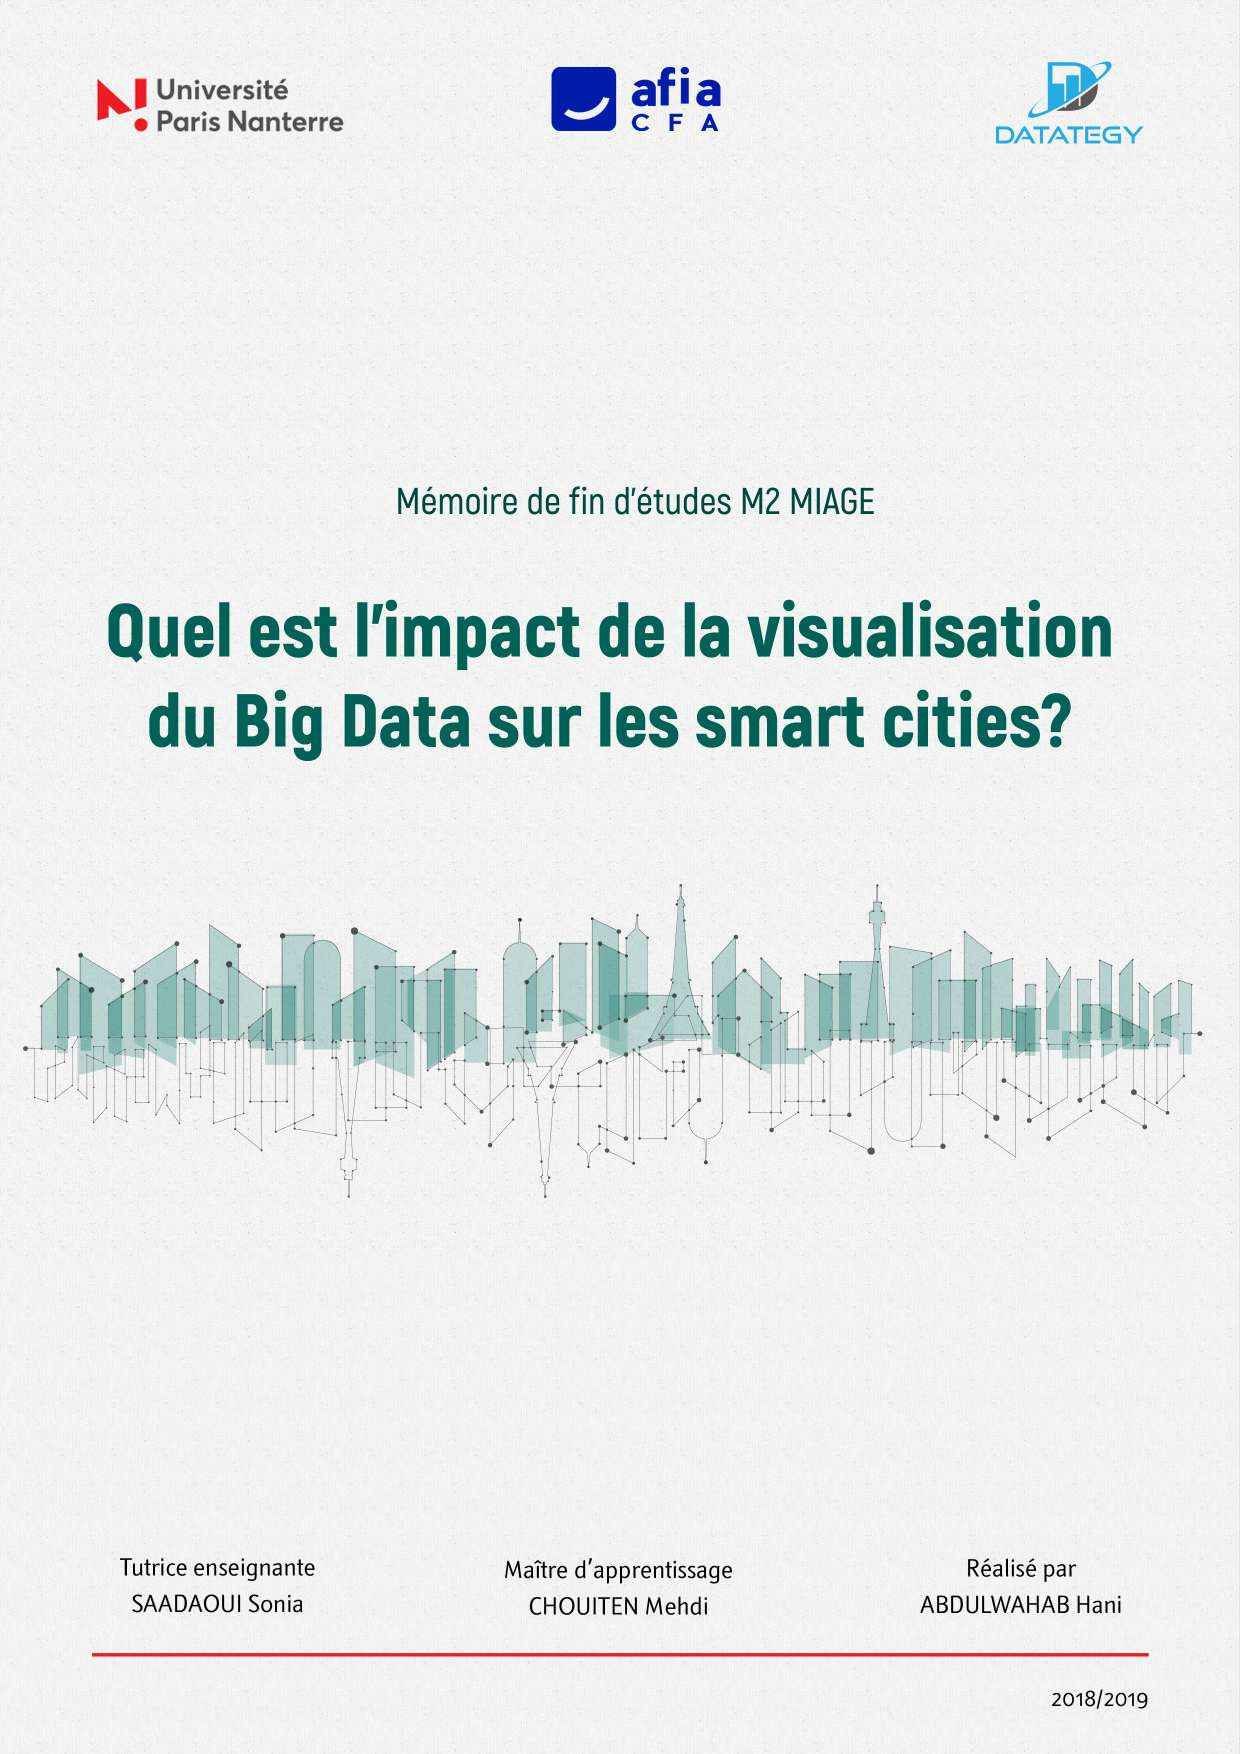
\includepdf{images/cover.pdf}
%\begin{titlepage}
%\begin{center}

%\begin{figure}[!htb]
%\minipage{0.25\textwidth}
 % 
\includegraphics[width=\linewidth]{images/parisNanterre-logo}
%\endminipage\hfill
%\minipage{0.2\textwidth}
 % 
\includegraphics[width=\linewidth]{images/logo_afia_2x.png}
%\endminipage\hfill
%\minipage{0.2\textwidth}%
%  
\includegraphics[width=\linewidth]{images/datategy.png}
%\endminipage
%\end{figure}
%\vspace{1cm}
%{\Large Mémoire de fin d'étude Master 2 MIAGE}\\[0.5cm]


% Title
%\rule{\linewidth}{0.5mm} \\[0.4cm]
%{ \huge \bfseries Quel est l'impact de la visualisation du Big Data sur les smart cities? \\[0.4cm] }
%\rule{\linewidth}{0.5mm} \\[1.5cm]
%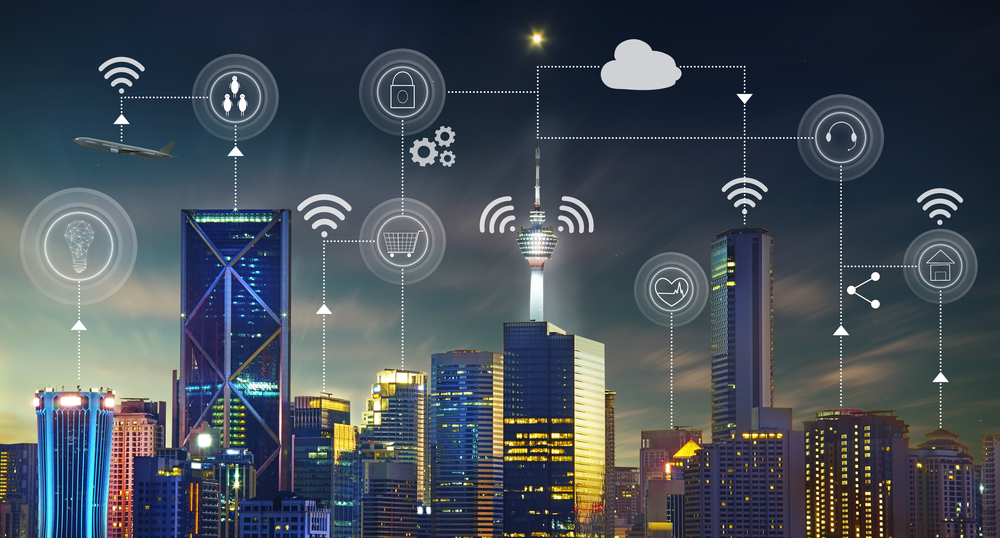
\includegraphics[width=1\textwidth]{images/Smart-City.jpg}\\[1cm]
% Author and supervisor
%\noindent
%\begin{minipage}{0.4\textwidth}
%  \begin{flushleft} \large
%    \emph{Étudiant :}\\
%    Hani \textsc{Abdulwahab}
%  \end{flushleft}
%\end{minipage}%
%\begin{minipage}{0.4\textwidth}
%  \begin{flushright} \large
%    \emph{Encadrants :} \\
%    Mme.~Sonia \textsc{GUEHIS}\\
%    M.~Mehdi \textsc{CHOUITEN }

%  \end{flushright}
%\end{minipage}
%
%\vfill

% Bottom of the page
%{\large Version 1.0 du\\ \today}

%\end{center}
%\end{titlepage}

\tableofcontents
\listoffigures
\chapter*{Remerciements}

\chapter*{Introduction}
\addcontentsline{toc}{chapter}{Introduction}
Une ville intelligente idéale est une ville où l’on peut mener une vie saine et agréable, avec à disposition des moyens de transport fiables. Une ville intelligente, en tant qu’organisme vivant, vérifie ses fonctions vitales, s’ajuste et se maintient saine, minimisant ainsi les inconvénients de l’urbanisation. Loin des embouteillages, des pénuries de logements, des concentrations malsaines de poussière fine, des centres-villes surpeuplés, des structures sociales en ruine et du bruit.
L'expansion du Big Data et l'évolution des technologies de l'Internet des objets (IoT) ont joué un rôle important dans la faisabilité des initiatives de ville intelligente. Les mégadonnées offrent aux villes la possibilité d’obtenir des informations précieuses à partir d’un grand nombre de données recueillies auprès de diverses sources, et l’Internet des objets permet l’intégration de capteurs, d’identification par radiofréquence et de Bluetooth dans un environnement réel utilisant des services hautement interconnectés. La combinaison de l'IoT  et du Big Data est un domaine de recherche inexploré qui a apporté de nouveaux défis intéressants pour atteindre l'objectif des futures villes intelligentes. Ces nouveaux défis se concentrent principalement sur des problèmes liés aux technologies qui permettent aux villes d’actualiser la vision, les principes et les exigences des applications des villes intelligentes en réalisant les principales caractéristiques de l’environnement intelligent.
Les smart cities sont le futur des grandes villes et les entreprises doivent décider de comment gérer les données et comment permettre à ses parties prenantes de prendre des décisions. 
%La flexibilité et la rapidité seront les critères qui obligeront ces entreprises à tendre vers la visualisation Big Data.
Les données sont toujours plus nombreuses, plus complexes, plus variées et donc plus volumineuses, et plus particulièrement dans le cas des Smart Cities. 
Comment les analyser et en tirer profit pour prendre la meilleures décision au sein d’une entreprise et stimuler sa croissance ? 
%Pour répondre à cette problématique “Une image vaut mieux que mille mots”.
La visualisation de données est la présentation de données dans un format graphique. Il permet aux décideurs de voir les analyses présentées de manière visuelle, afin de pouvoir comprendre mieux et d’identifier de nouveaux modèles. 
Pour la business intelligence, la visualisation des données est très utile. Au lieu de parcourir un rapport comportant des centaines de lignes, un utilisateur professionnel peut simplement consulter un graphique.
Pour les Smart cities, elles apparaissent comme une stratégie de gestion de la performance urbaine. Pour ce processus, il est nécessaire de visualiser un grand nombre de paramètres, souvent en temps réel. 
La visualisation des données est devenue un centre d'intérêt pour la recherche, les industries, les gouvernements et les autres organisations pour améliorer la mobilité, l'efficacité énergétique, la gestion des déchets et l'administration publique d'une ville intelligente. Les exigences du Big Data, les volumes croissants, les formats et normes de qualité variables, présentent des défis pour la gestion, le stockage, la visualisation et l'analyse des données, telles que la Geo-Visualisation et la Visual Analytics des données géospatiales. Celles-ci sont collectées dans une ville intelligente et permettent de décrire le potentiel de telles techniques. Cela aidera à mieux comprendre le système urbain et à permettre le développement durable des villes futures en améliorant les interactions humaines avec les données géospatiales.

Dans le cadre de mon Master M2 MIAGE à l’Université Paris Nanterre, j’ai souhaité réaliser cette mémoire sur l'impact de la visualisation du Big Data sur les smat cities. 
%En effet, j’ai effectué au cours de mes études d’ingénieur en Télécommunication un mémoire sur la reconnaissance sonore qui permettait de visualiser le son avec une image. Ce mémoire m’a fait découvrir l’intérêt de la visualisation. 
Actuellement, le contexte des villes modernes souhaitant devenir des villes intelligentes met en valeur la visualisation comme moyen d’analyse des données. L’enjeu est important pour des entreprises comme Datategy où j’effectue mon alternance en tant que développeur web front-end. J’ai eu de nombreuses tâches sur la visualisation du Big Data dans le cadre d’une Smart City. Les réalisations effectuées grâce à la visualisation du Big Data, l’utilisation de différentes techniques  et outils m’intéressent particulièrement. 

Dans un premier temps, la définition théorique de la ville intelligente sera présenté. Cette définition se veut être un idéal vers lequel la ville intelligente veut tendre. L’impact de l'évolution des Smart Cities sur les domaines de l’économie, de la gouvernance, de l’environnement, de la mobilité et de la démographie seront analysés. Puis, le rôle de la technologie dans les Smart Cities telles que les données numériques (Big Data) et l’Internet of Things (IoT) sera abordé. Puis, la visualisation du Big Data, ses défis ainsi que les techniques et les outils de visualisation de données sera présentés. 
Dans un second temps, la réalisation d’une étude comparative entre les différentes techniques et outils présentés dans le chapitre précédent. 
Dans un troisième temps, nous décrirons un cas pratique :  la visualisation du Big Data chez Datategy. 
Finalement, un bilan professionnel et personnel sera présenté. 

\chapter{Smart city  et  visualisation du Big Data}
\section{Smart city}
\subsection{Définition de la ville intelligente}
\subsubsection{Historique:}
La croissance des villes depuis la révolution industrielle a atteint des niveaux sans précédent. 
%La division de la population des Etats-Unis a estimé qu'en 2016, 54,5\% de la population mondiale vivait dans des zones urbaines et qu'en 2050, ce nombre atteindrait 67\% \cite{0}. 
Cette croissance considérable de la population urbaine nécessitera d’importants développements d’infrastructures urbaines pour faire face à la demande de ses habitants. Il ne fait aucun doute que les villes sont des systèmes complexes et que la croissance urbaine rapide engendre des embouteillages, une pollution et une inégalité sociale croissante. Ceux-ci peuvent transformer la ville en un point de convergence de nombreux risques (économiques, démographiques, sociaux et environnementaux). Cela pourrait sérieusement dépasser leur capacité à fournir des services adéquats à leurs citoyens \cite{1}. Cependant, des villes bien gérées peuvent offrir de multiples avantages aux personnes qui y vivent car elles permettent de réaliser des économies d’échelle en partageant des commodités telles que les transports, les installations de sport et de divertissement, les services aux entreprises, le haut débit, etc.
Depuis les années 1990, les gouvernements et les chercheurs utilisent le terme « villes intelligentes » comme un label de mode ou pour aider certaines villes à se distinguer et à se promouvoir comme innovantes. Être une ville intelligente est une aspiration pour certaines villes qui ont élaboré des plans à long terme afin d’atteindre cet objectif. Le terme ville intelligente est considéré comme un anthropomorphisme (attribution de caractéristiques humaines à la ville), car il repose sur la capacité de la ville à détecter et à relever ses défis de manière intelligente, en utilisant une intelligence naturelle et artificielle intégrée aux systèmes d’information de la ville \cite{2}.
\subsubsection{Définition:}
De nombreuses études ont tenté de définir le concept de ville intelligente, mais le défi reste difficile à relever. C’est un concept multidisciplinaire et il est difficile de définir le terme « intelligent ». Les premières tentatives de définition du concept ont été axées sur l'intelligence des technologies de l'information pour la gestion de diverses fonctions de la ville \cite{3}. 
Dernièrement, les études ont élargi leur champ d'action en incluant les résultats de la ville intelligente tels que la durabilité, la qualité de vie et les services aux citoyens.
L'évaluation du niveau d'intelligence des villes est également devenue importante pour les chercheurs et les responsables gouvernementaux. Ils ont développé des classements prenant en compte des variables telles que l'économie, les infrastructures, l'innovation, la qualité de vie, les transports, le développement urbain, etc. \cite{4}.
Malgré la vaste littérature sur les villes intelligentes, il existe plus de trente définitions du terme. Ils abordent des aspects différents, mais pertinents, notamment la construction de ces villes \cite{5}. 
Il ne fait aucun doute qu'une ville intelligente est un concept multidisciplinaire qui englobe non seulement son infrastructure informatique, mais également sa capacité à gérer les informations et les ressources pour améliorer la qualité de vie de ses habitants. L'utilisation de la technologie de l'information est considérée comme un facteur clé de l'intelligence d'une ville, car elle peut détecter, surveiller, contrôler et communiquer la plupart des services de la ville tels que les transports, l'électricité, le contrôle de l'environnement, la lutte contre la criminalité, les urgences sociales, etc \cite{6}.
\subsection{Étapes pour la mise en œuvre de projets de ville intelligente}

La mise en œuvre réussie d'un projet de ville intelligente nécessite la mise au point d'un système numérique capable de gérer et de visualiser les données géospatiales dans un environnement convivial. Le système d'information géographique (SIG) offre des fonctionnalités avancées et convivial pour les projets de ville intelligente.
Le concept de « ville intelligente » vise à développer un système complet qui utilise des données géospatiales pour améliorer la compréhension des systèmes urbains complexes et pour améliorer l’efficacité et la sécurité de ces systèmes. 
Ces données géospatiales concernent :
\begin{itemize}
\item \textbf{} L’environnement urbain construit tel que les infrastructures, les bâtiments et les espaces publics.
\item \textbf{} L’environnement naturel tel que la biodiversité, les espaces verts, la qualité de l’air, le sol et l’eau.
\item \textbf{} Les services urbains tels que les transports, les déchets municipaux, l’eau, l’énergie, la santé et l’éducation. 
\end{itemize} 
Le concept de ville intelligente vise également à transformer la gestion des villes «en silo» en un système «partagé» impliquant les acteurs urbains dans la conception, la réalisation et l’évaluation de projets urbains.
\begin{figure}[!ht]
    \centering
    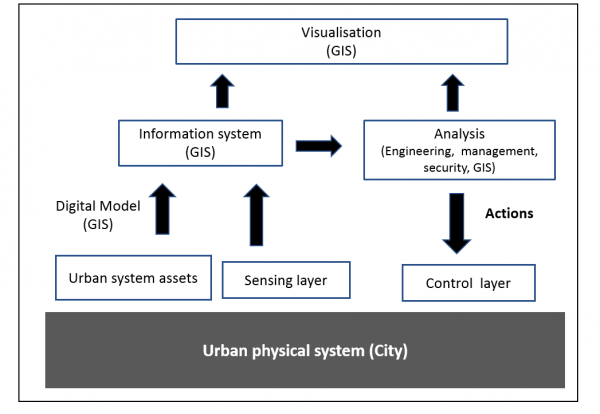
\includegraphics[height=8cm]{images/Steps.png}
    \scriptsize{source :}
    \caption{Étapes pour la mise en œuvre d’un projets de ville intelligente}
    \label{fig:2.1}
\end{figure}
Figure~\ref{fig:2.1} inclut la construction du modèle numérique urbain, la collecte de données à l'aide de la couche de détection, puis l'analyse des données, la visualisation interactive des données et le contrôle du système. Le SIG joue un rôle dans ces étapes, comme décrit ci-dessous. 

\subsubsection{1. Construction du modèle de ville intelligente:}
La première étape de la mise en œuvre d’un projet de ville intelligente concerne la construction du modèle numérique urbain qui décrit les composants des environnements urbains et naturels construits. Le modèle numérique fournit pour chaque composant urbain la géolocalisation et les caractéristiques (attributs). Les SIG sont généralement utilisés pour la construction du modèle numérique de «composants horizontaux» urbains tels que les réseaux urbains, les installations de transport et l’environnement naturel, tandis que la modélisation des données du bâtiment (BIM) est utilisée pour la description de «composants verticaux» tels que les bâtiments. La combinaison des SIG et du BIM fournit un outil puissant pour la construction du modèle numérique urbain avec des données géoréférencées et la visualisation de ces données dans un environnement convivial.

\subsubsection{2. Couche de détection:}
La deuxième étape d’un projet de ville intelligente concerne la construction de la couche de détection qui transfère les données d’exploitation urbaine au système d’information de la ville intelligente. Cette couche comprend des capteurs utilisés pour la surveillance des réseaux et infrastructures urbains. Les données pourraient également être enrichies d'images, de vidéos et de fichiers audio, ce qui aboutirait à la construction de mégadonnées urbaines. Par exemple le système d'eau potable utilise des lecteurs de compteurs automatiques (AMR) pour enregistrer la consommation d'eau, des capteurs de pression pour enregistrer la pression de l'eau et des dispositifs de contrôle de la qualité de l'eau permettant de suivre la qualité de l'eau (turbidité, pH, chlore, conductivité). Le système de drainage utilise des capteurs pour surveiller le niveau et le débit d'eau, la qualité de l'eau (turbidité, température, pH, etc.) et le matériel de pompage. Il permet une détection précoce des inondations et des défauts dans les équipements de pompage. Le réseau électrique utilise des capteurs pour mesurer la tension électrique, le courant et la fréquence. Il permet une détection précoce des défauts du réseau électrique. Le système de chauffage urbain est surveillé par des capteurs pour enregistrer la température, la pression et le débit du fluide, ainsi que l'état de la vanne. Il permet la détection précoce des pannes et l'amélioration des performances du système. Le SIG offre la possibilité de visualiser le système de surveillance ainsi que les caractéristiques et l’état des capteurs. Il offre également la possibilité de visualiser des données historiques et en temps réel sur des cartes SIG.
\subsubsection{3. L'analyse des données:}
La troisième étape de la mise en œuvre d'un projet de ville intelligente concerne le développement d'un environnement analytique, qui transforme les données en temps réel améliorant la sécurité, l'efficacité et la qualité des systèmes urbains. L'environnement analytique comprend des logiciels d'ingénierie, de gestion et de sécurité pour les systèmes urbains, ainsi que des outils numériques avancés tels que l'intelligence artificielle (IA). Dans les projets de ville intelligente, les SIG fournissent des outils pour (i) l’analyse de données géospatiales (traitement géométrique, modèles de grille), (ii) l’analyse spatio-temporelle, (iii) les statistiques spatiales (autocorrélation spatiale et modèle de régression), (iv) l’analyse de surface (analyse de la forme et du flux de surface, méthodes de maillage et d'interpolation) et (v) analyse de localisation (calcul du plus court chemin, localisation de l'installation).

\subsubsection{4. Visualisation interactive des données:}
La visualisation interactive des données permet aux utilisateurs d’interagir avec les composants de la ville intelligente et les parties prenantes (Skateholder) dans un environnement convivial. Les applications Web sont utilisées pour créer cet environnement interactif. L'utilisation de fenêtres contextuelles HTML permet aux utilisateurs d'accéder à du contenu Web, tel que des graphiques référencés par des URL. L'environnement graphique SIG interactif permet la visualisation de composants urbains et de cartes de capteurs. Les utilisateurs et les gestionnaires peuvent utiliser ces cartes pour accéder aux données statiques et dynamiques concernant les systèmes urbains ainsi que pour mettre à jour les données.

\subsubsection{5. Couche de contrôle}
L'analyse des données en temps réel et des données historiques donne lieu à des commandes pour une gestion optimale et sécurisée des systèmes urbains. Ces commandes sont transmises à la couche de contrôle, qui comprend différents dispositifs électroniques tels que des vannes intelligentes, des pompes, des moteurs, des commutateurs, des disjoncteurs et des serrures. Le système SIG permet une visualisation en temps réel de ces appareils ainsi que de leur statut. Il pourrait également visualiser les erreurs dans la commande de l'appareil.
%%%%%%%%%%%%%%%%%%%%%%%%%%%%%%%%%%%%%%%%%%%%%%%%%%%%%%%%%%%%%%%%%%%%%%%
\subsection{Avantages et opportunités}
Les avantages d’une ville intelligente sont notamment les suivants [9] :
\begin{itemize}
\item \textbf{}Amélioration de la qualité de vie des citoyens.
\item \textbf{}Mise en place d’une gestion intelligente des infrastructures et des ressources naturelles.
\item \textbf{}Utilisation efficace des ressources avec les systèmes technologiques tels que la planification des ressources d'entreprise (ERP) et le système d'information géographique (SIG) [9].
\item \textbf{}Meilleure qualité de vie pour les citoyens : grâce à des services plus rapides, moins coûteux en temps et en énergie, à une meilleure planification des espaces et des lieux de vie et de travail, à des transports plus efficaces et à la disponibilité des informations concernant la ville pour les citoyens. 
\item \textbf{}Niveaux plus élevés de transparence et d’ouverture : le partage des données et des ressources, la transparence de l'information pour toutes les personnes impliquées encourage la collaboration et la communication entre entités et la création de plus de services et d'applications améliorant davantage la ville intelligente.
\end{itemize}
%%%%%%%%%%%%%%%%%%%%%%%%%%%%%%%%%%%%%%%%%%%%%%%%%%%%%%%%%%%%%%%%%%%%%%%
\section{Le rôle de la technologie dans les smart cities}
\subsection{Les données numériques (Big Data) }
Les applications Big Data peuvent potentiellement servir de nombreux secteurs dans une ville intelligente. Elles aident à fournir de meilleures expériences client et de meilleurs services, ce qui aident les entreprises à améliorer leurs performances. Améliorer les soins de santé en améliorant les services de soins préventifs, les outils de diagnostic et de traitement, la gestion des dossiers de santé et les soins aux patients. Les systèmes de transport peuvent grandement tirer parti des données volumineuses pour optimiser les itinéraires et les horaires, répondre aux demandes variées et être plus respectueux de l'environnement.
Le déploiement d’applications Big Data nécessite la mise en place d’une bonne infrastructure de technologies de l’information et de la communication (TIC). Les TIC soutiennent les villes intelligentes car elles apportent des solutions utiles, ainsi que des solutions uniques qui ne seraient peut-être pas possibles sans elles.
L’adoption de solutions TIC, Cloud et Big Data aide à résoudre de nombreux problèmes, tels que la fourniture des outils de stockage et d’analyse. En outre, cela aide à atteindre le stade de l'innovation et encourage la collaboration et la communication entre les différentes entités d'une ville intelligente.
Il existe de nombreux exemples d'applications Big Data servant les villes intelligentes telles que:
\begin{itemize}
\item \textbf{}Education intelligente [10]: les TIC offrent une solution pour améliorer l'efficience, l'efficacité et la productivité des processus éducatifs grâce à des services éducatifs intelligents et flexibles permettant une meilleure utilisation de l'information, un contrôle et une évaluation améliorés, un soutien accru à l'apprentissage pour tous et tout au long de la vie. Les applications pédagogiques intelligentes impliquent les utilisateurs dans des environnements d’apprentissage actifs leur permettant de s’adapter aux changements rapides de la société et de l’environnement. Les mégadonnées dans l'éducation sont générées principalement par la collecte de données sur des personnes (par exemple des élèves, des enseignants, des parents, des administrateurs et d'autres personnels de soutien), des infrastructures (par exemple des écoles, des bibliothèques, des installations informatiques, des lieux d'enseignement, des musées et des universités) et des informations (cours, livres, examens, notes, enquêtes économiques, évaluations, rapports, etc.). 
\item \textbf{}Feux de circulation intelligents [11]: L’un des principaux aspects des villes intelligentes est un bon contrôle de la circulation dans la ville, ce qui améliore les systèmes de transport et les déplacements des citoyens ainsi que la structure générale du trafic des villes. L'utilisation de feux de signalisation intelligents et de signaux est l'une des techniques les plus importantes que les villes intelligentes utilisent pour faire face aux volumes de trafic et aux encombrements élevés. Les feux de signalisation intelligents et les signaux doivent être interconnectés sur les réseaux routiers pour offrir plus d'informations sur les schémas de trafic. Chaque capteur détecte un paramètre différent du flux de trafic (par exemple, la vitesse des voitures, la densité du trafic, le temps d'attente aux feux, les embouteillages, etc.). Le système prend des décisions en fonction des valeurs de ces paramètres et donne les instructions appropriées aux voyants et aux signaux. 
\item \textbf{}Réseau intelligent: un réseau intelligent utilise des télécommandes informatiques avec une technologie de communication bidirectionnelle entre les producteurs d'électricité et les consommateurs afin d'accroître l'efficacité et la fiabilité du réseau grâce à l'auto-surveillance et à la rétroaction du système. Cela implique de placer des capteurs et des compteurs intelligents sur les systèmes de production, de transmission et de distribution en plus des points d'accès des consommateurs pour obtenir des données granulaires en temps quasi réel sur la production, la consommation et les défauts actuels. Le traitement des données collectées, considérées comme une analyse de données volumineuses, en temps réel permet de renvoyer certaines informations de contrôle afin d'améliorer les performances globales du système d'alimentation électrique.
Cela permet la mise en oeuvre des modèles de tarification dynamiques pour la consommation d'énergie, d’éviter les pannes d’électricité potentielles dues à la forte demande des consommateurs et peut fournir aux consommateurs des informations en temps quasi réel sur leur consommation d'énergie et de faire fonctionner leurs appareils pendant les périodes de tarification plus basse. 

\end{itemize}


\subsection{Internet of Things (IoT)}
L'Internet des objets (IoT) est ce qui garde tout connecté dans la ville. IoT offre une connectivité avancée des appareils intelligents, des appareils portables, des appareils et des services domestiques intelligents, des appareils médicaux, des véhicules connectés, des divertissements intelligents, des bâtiments intelligents, une mobilité publique intelligente, une agriculture intelligente, une infrastructure de ville intelligente et tous les systèmes et services allant au-delà de la simple machine (communication machine M2M).
L'IoT fournit le corps de périphériques en communication. Un écosystème IoT se compose d’appareils intelligents activés sur le Web qui utilisent des processeurs, des capteurs et du matériel de communication intégrés pour collecter, envoyer et exploiter les données acquises dans leurs environnements. 
Les périphériques IoT partagent les données des capteurs qu'ils collectent en se connectant à une passerelle IoT ou à un autre périphérique, où les données sont envoyées au cloud pour être analysées ou sont analysées localement. Parfois, ces appareils communiquent avec d’autres appareils apparentés et agissent en fonction des informations qu’ils obtiennent les uns des autres. Les appareils effectuent la majeure partie du travail sans intervention humaine, bien que les utilisateurs puissent interagir avec eux, par exemple pour les configurer, leur donner des instructions ou accéder aux données.

Les protocoles de connectivité, de mise en réseau et de communication utilisés avec ces périphériques Web dépendent largement des applications IoT spécifiques déployées.

L'IoT offre de nombreux avantages aux organisations, leur permettant de:
\begin{itemize}
\item \textbf{}Surveiller leurs processus d'affaires globaux. 
\item \textbf{}Améliorer l'expérience client.
\item \textbf{}Gagner du temps et de l'argent. 
\item \textbf{}Améliorer la productivité des employés. 
\item \textbf{}Intégrer et adapter les modèles d'entreprise. 
\item \textbf{}Prendre de meilleures décisions d'affaires. 
\item \textbf{}Générer plus de revenus.
\end{itemize}
L'IoT encourage les entreprises à repenser leur façon d'aborder leurs activités, leurs industries et leurs marchés et leur donne les outils nécessaires pour améliorer leurs stratégies commerciales.
\begin{figure}[!ht]
    \centering
    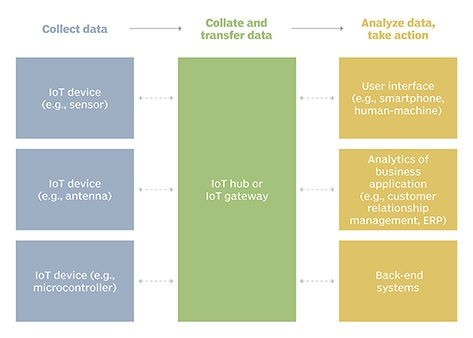
\includegraphics[height=9cm]{images/iot_system.jpg}
    \scriptsize{source :\url{https://internetofthingsagenda.techtarget.com/}}
    \caption{Exemple d'un systéme IoT}
    \label{fig:1.2}
\end{figure}
%%%%%%%%%%%%%%%%%%%%%%%%%%%%%%%%%%%%%%%%%%%%%%%%%%%%%%%%%%%%%%%%%%%%%%%
\subsection{Avantages du Big Data dans les composants de la ville intelligente}
\subsubsection{La smart gouvernance:}
La smart gouvernance soutient l'intégration et la collaboration de différentes agences gouvernementales et combine ou rationalise leurs processus. Cela se traduit par des opérations plus efficaces, un meilleur traitement des données partagées, une gestion et une application plus stricte de la réglementation.
Elle améliore les décisions commerciales grâce au support d'analyse Big Data. En recherchant le comportement et la croissance économique d’une entreprise en plus de ses concurrents et des conditions environnementales, les prises de décisions sont plus appropriées et plus efficaces en matière d’emploi, de production et de stratégies de localisation.
Elle permet la publication de nouvelles politiques au profit des propriétaires de données (citoyens) et des producteurs (agences gouvernementales). Les agences gouvernementales aident à développer la qualité des données, tandis que les citoyens montrent comment ils peuvent utiliser les données et les transférer vers de nouvelles connaissances afin d'améliorer la qualité des services publics.
Elle aident les gouvernements à se concentrer sur les préoccupations des citoyens en matière de santé et de protection sociale, de logement, d’éducation, de police et autres.\\
\subsubsection{Le smart environnement :}
Le smart environnement fournit des informations météorologiques qui permettront d’améliorer l’agriculture du pays, de mieux informer la population sur les conditions potentiellement dangereuses et de mieux gérer l’utilisation de l’énergie en fournissant des prévisions plus précises à la demande.\\
\subsubsection{La smart mobilité :}
La smart mobilité reconnaît les modèles de trafic en explorant les données en temps réel. 
Elle réduit les embouteillages sur les routes principales de la ville en prévoyant les conditions de circulation et en ajustant les contrôles de circulation. Grâce au Big Data, la ville intelligente peut réduire le trafic et les accidents en ouvrant de nouvelles routes, en améliorant l'infrastructure en fonction des données de congestion et en collectant des informations sur le parking et les routes alternatives.
Elle réduit les déchets de la chaîne d'approvisionnement en associant les livraisons et en optimisant les mouvements d'expédition.
Elle active la transmission en continu des données pour traiter et communiquer aux conducteurs les informations sur le trafic collectées via des capteurs, des feux de signalisation intelligents et des dispositifs embarqués via des smartphones ou d'autres dispositifs de communication.
Les mégadonnées peuvent être utilisées pour envoyer des informations en retour à des entités spécifiques afin qu’elles prennent des mesures visant à atténuer ou à résoudre un problème de trafic.\\
\subsubsection{La smart énergie:}
La smart énergie facilite la prise de décision concernant les niveaux d'approvisionnement en électricité en adéquation avec la demande réelle des citoyens et dans toutes les conditions qui affectent.
Elle permet la prévision en temps quasi réel grâce à une analyse efficace des données volumineuses collectées.
Elle s’aligne sur les objectifs stratégiques (optimisation des ressources) par le biais de plans de tarification spécifiques compatibles avec les modèles d'approvisionnement, de demande et de production.\\
\subsubsection{La smart éducation:}
La smart éducation optimise la recherche universitaire. Par exemple, l'astronome peut maintenant analyser un grand ensemble de données astronomiques en utilisant des ordinateurs puissants au lieu d'analyses manuelles. En analysant et en explorant des images numériques de haute qualité prises depuis l'espace, de nouvelles découvertes peuvent se produire sur le terrain. Cela s'applique à de nombreux domaines scientifiques et de recherche tels que les expériences médicales, les opérations de fabrication, les études environnementales et les analyses économiques et financières.
Le comportement et le jumelage mèneront à de nouvelles connaissances. De l'évaluation des diplômés aux attitudes en ligne, chaque élève génère un suivi de données unique. En analysant ces données, les établissements d’enseignement peuvent déterminer s’ils utilisent leurs ressources aux bons endroits et produisent les bons résultats.\\
\subsubsection{La smart sécurité:}
La smart sécurité fournit des cartes des zones géographiques détaillées sur le plan spatial et le plan temprel, permettant ainsi d’aider à déterminer facilement les changements qui pourraient survenir.
Elle aide à prévoir les changements environnementaux futurs ou les catastrophes naturelles telles que la détection des tremblements de terre, qui permettront de sauver des vies et d'économiser des ressources.\\

\subsection{Les exigences des applications de ville intelligente}
Les applications de ville intelligente basées sur le Big Data doivent répondre à plusieurs exigences découlant de la nature particulière des besoins de la ville intelligente et des caractéristiques du Big Data. Certaines exigences sont technologiques, tandis que d’autres sont liées à la sensibilisation des citoyens et aux rôles des gouvernements.\\
\subsubsection{Gestion des données volumineuses : }
Le principal avantage des applications de ville intelligente est qu’elles génèrent de gros volumes de données dans divers formats et dans de nombreux secteurs tels que le trafic, l’énergie, l’éducation, la santé et la fabrication. Ces données sont générées et collectées de manière massive et régulière, offrant ainsi une vue en temps réel de ce qui se passe dans la ville à tout moment. Pour garantir une utilisation appropriée et utile de ces données dans les applications de ville intelligente, il est important de disposer d'outils de gestion des données volumineuses appropriés et efficaces. La gestion des données volumineuses comprend le développement et l'exécution d'architectures, de politiques, de pratiques et de procédures qui gèrent correctement l'ensemble du cycle de vie des données tout au long de son utilisation dans les applications de ville intelligente. Comme les données proviennent de sources différentes avec des formats différents, il est nécessaire de disposer de fonctionnalités avancées de gestion des données permettant de reconnaître les différents formats et sources de données, de structurer, de gérer, de classer et de contrôler tous ces types et structures. La gestion des données volumineuses pour les applications de ville intelligente doit également permettre une gestion évolutive de données volumineuses afin de prendre en charge les applications hors ligne, ainsi qu'un traitement à faible temps de latence pour servir efficacement les applications en temps réel.\\
\subsubsection{Plateformes de traitement de données volumineuses:}
Les applications Big Data pour les villes intelligentes doivent effectuer des analyses de données qui nécessitent généralement une capacité de traitement énorme. Cela conduit à la nécessité de disposer des plateformes matérielles et logicielles évolutives et fiables. Les plateformes logicielles pour les villes intelligentes doivent offrir des capacités de calcul hautes performances, être optimisées pour le matériel utilisé, être stables et fiables pour les différentes applications nécessitant des données en cours d'exécution, prendre en charge le traitement de flux, fournir des niveaux élevés de résilience aux pannes et soutenu par une équipe et un fournisseur bien formés et compétents. Il existe différentes plateformes logicielles d'analyse des données volumineuses, telles que Hadoop Mapreduce , HPCC, Stratosphere et IBM Infosphere Streams, qui fournissent le traitement de flux requis par les applications de données volumineuses en temps réel. Ces plateformes fonctionnent bien sur des systèmes en cluster capables de fournir une plateforme matérielle, puissante et évolutive pour répondre aux exigences des applications de données volumineuses. Les mégadonnées peuvent également être traitées sur le Cloud en utilisant à la fois une plateforme Big Data (PaaS) et une infrastructure IaaS.\\
\subsubsection{Infrastructure de réseau intelligent:}

La plupart des applications Big Data pour les villes intelligentes exigent des réseaux intelligents connectant leurs composants, y compris les équipements des résidents, tels que les voitures, les appareils intelligents et les téléphones intelligents. Ce réseau doit être capable de transférer efficacement les données collectées de leurs sources vers le lieu de collecte, de stockage et de traitement des données volumineuses, ainsi que de renvoyer les réponses aux différentes entités qui en ont besoin dans la ville intelligente. La prise en charge de la qualité de service (QoS) sur le réseau est extrêmement importante pour les applications Big Data en temps réel destinées aux villes intelligentes. \\
\subsubsection{Algorithmes avancés:}
Les algorithmes standards utilisés dans les applications classiques peuvent ne pas être suffisants ou efficaces pour gérer les applications de données volumineuses en raison de leurs exigences spécifiques et de la nécessité impérieuse d'un traitement à grande vitesse et à haut volume. Les applications de données volumineuses pour les villes intelligentes doivent mettre en œuvre des algorithmes avancés et plus sophistiqués pour traiter efficacement les données volumineuses. Certains de ces algorithmes doivent être conçus pour la prise en charge d'applications en temps réel, tandis que d'autres peuvent être conçus pour un traitement par lots ou hors ligne. Ces algorithmes doivent être optimisés pour gérer des volumes de données élevés, une grande variété de types de données, des contraintes de temps sur les processus de prise de décision et des composants distribués sur divers emplacements géographiques. De plus, ces algorithmes doivent fonctionner efficacement dans des environnements hétérogènes et être capables de gérer et de fonctionner dans des environnements hautement dynamiques.\\
\subsubsection{Sécurité et confidentialité:}
Étant donné que la plupart des données collectées et traitées dans les applications de ville intelligente contiennent une forme d’information confidentielle, il est important de veiller à ce que tous les composants de la technologie et des applications incluent et maintiennent des niveaux acceptables de mécanismes de sécurité et de confidentialité. Bien qu'une ville intelligente offre de nombreux avantages positifs à ses résidents, elle fait peser de nombreuses menaces sur leur sécurité, leur bien-être et leur vie privée en s'appuyant fortement sur leurs données. La possibilité d'accès illégal ou d'attaques malveillantes à de telles infrastructures peut entraîner des résultats catastrophiques pour l'infrastructure de la ville, ses entités gouvernementales et ses résidents. Les concepteurs et les développeurs d’applications Big Data doivent inclure les politiques et les procédures de sécurité et de confidentialité, dans la conception et la mise en œuvre de leurs applications. \\
\subsubsection{Sensibilisation des citoyens:}
Les citoyens doivent savoir utiliser correctement et en toute sécurité les solutions TIC pour une ville intelligente. Leur participation active au gain d'informations sur les différents problèmes rencontrés avec les applications de ville intelligente contribue à améliorer la qualité des données collectées et la performance des applications. Un autre aspect important de la sensibilisation des citoyens est leur connaissance et leur usage de bonnes pratiques en matière de sécurité et de protection de la vie privée. \\
\subsubsection{Rôle du gouvernement:}
Les entités gouvernantes des villes intelligentes doivent établir des principes directeurs d'ouverture, de transparence, de participation et de collaboration afin de contrôler les échanges et le flux de données volumineuses [14]. Les gouvernements jouent un rôle essentiel dans une ville intelligente. Le gouvernement doit revoir et réajuster les politiques en matière d'informations et de données, en fonction des besoins, en mettant l'accent sur la confidentialité, la réutilisation des données, la précision des données, l'accès aux données, leur archivage et leur conservation [14]. 
Pour prendre en charge efficacement les applications de données volumineuses, le gouvernement des villes intelligentes doit établir un équilibre entre les utilisations bénéfiques des données et les préoccupations des particuliers en matière de vie privée, en abordant certains des concepts fondamentaux des lois sur la vie privée.\\


\section{Visualisation du Big Data }
\subsection{Context}
Les villes cherchent à devenir intelligentes en connectant les systèmes isolés des organismes municipaux et en installant des capteurs intelligents. Les administrateurs de la ville cherchent à exploiter les informations tirées des données des capteurs de l'Internet des objets (IoT), de systèmes de positionnement global (GPS), de smartphones et d'ordinateurs. 80\% de ces données sont des données sombres, ce qui signifie que les données sont non structurées pour transmettre un sens en soi.
Il est important de visualiser les données traitées pour découvrir les modèles et pour décider les prochaines étapes. Dans le but de faire ce processus efficacement, il est extrêmement important que les décideurs puissent visualiser et interagir avec les données.
Cela signifie qu'il est possible de supprimer la dépendance sur des experts en données de la boucle, ce qui signifie aussi que la plateforme de visualisation de données doit être interactive pour interagir avec les données, donc les idées deviennent visuellement évidentes dans le processus de découverte.

\subsection{L’importance de la visualisation du Big Data}
La visualisation de données, qui exploite la puissance de la réalité virtuelle, de la réalité augmentée et de l’apprentissage automatique, est une plateforme idéale pour la visualisation de flux de données IoT. La visualisation naturelle basée sur les gestes est non seulement intuitive, mais elle est également capable de montrer des données spatiales et temporelles complexes sur la réplique virtuelle d’un environnement, par exemple le modèle Google Earth ou le prototype 3D d’une ville.
La nouvelle technologie nous libère des cages de données à écran plat bidimensionnelles et nous permet de pénétrer dans nos données elles-mêmes en nous aidant à découvrir des informations grâce à un moyen de corrélation visuelle simpliste mais très puissant. Il n’est pas difficile de prendre des décisions avec la visualisation des données.
Plusieurs avantages plus spécifiques méritent d’être pris en compte. Voici quelques-uns des avantages les plus précieux de la visualisation de données volumineuses :
\subsubsection{1. Traiter rapidement de grandes quantités de données:}
Avec autant d’informations saisies, organisées et analysées, il y a tout simplement trop de données brutes pour que l’esprit humain moyen puisse les traiter à un rythme raisonnable. La visualisation de données volumineuses supprime le long processus de compréhension des données et permet aux utilisateurs de digérer rapidement des quantités de données volumineux et complexes. Ceci est souvent accompli par l’utilisation de tableaux de bord interactifs, présentés visuellement.
\subsubsection{2. Accéder aux données importantes en temps réel:}
Dans le monde des affaires au rythme rapide, chaque seconde compte. Les entreprises qui doivent s’appuyer sur des méthodes plus traditionnelles pour rassembler et affiner une grande quantité de données se retrouvent souvent avec des informations obsolètes. D'autre part, les meilleurs outils de visualisation de données volumineuses fonctionnent en temps réel et mettent constamment à jour les informations présentées. Ainsi, chaque fois qu'un utilisateur a besoin d'y accéder, il dispose toujours des données les plus récentes.
\subsubsection{3. Voir les liens entre les processus métier et les performances:}
Même si peu de dirigeants nieraient le fait que les processus et les activités opérationnels quotidiens d’une organisation aient un impact direct sur les performances globales de l’entreprise, il peut être difficile de voir exactement comment ces activités affectent le succès de la société. Les outils de visualisation de données volumineuses résolvent ce problème en permettant aux dirigeants de découvrir visuellement les relations cachées qui relient les processus quotidiens aux performances de l'entreprise.
\subsubsection{4. Raconter une histoire à travers des données:}
L'esprit humain a tendance à préférer traiter les informations de manière linéaire, c'est-à-dire qu'il aime voir les causes, les effets et les résolutions alignés de manière à raconter une histoire. En présentant les données de manière centrée visuellement, la visualisation de données volumineuses donne à l’information quelque chose qui lui manque généralement : un sentiment de progression. Cela rend la compréhension plus facile et l’utilisation aussi à utiliser pour les utilisateurs.
\subsection{Les éléments déterminant le choix de visualisation du Big Data:}
La visualisation est la première étape pour donner du sens aux données. Pour transcrire et présenter de manière simple les corrélations de données, les analystes de données utilisent un large éventail de charts, de diagrammes et de cartes. Le choix de la bonne technique et de sa configuration est souvent le véritable enjeu pour rendre les données compréhensibles. Et inversement, l’utilisation de techniques erronées peut ne pas présenter tout le potentiel des données, voire les rendre non pertinentes.

Les nombreux facteurs qui influencent les choix de visualisation des données sont :
\subsubsection{1. L’audience:}
Il est important d’ajuster la représentation des données au public cible. Par exemple, si ce sont des clients finaux qui parcourent leurs progrès dans une application de sport, la simplicité est de mise. Par contre, si les analyses de données sont destinées à des chercheurs ou à des décideurs expérimentés, il est nécessaire d’aller au-delà des simples graphiques.
Il faut décider les données que la visualisation affichera, quels sont ses objectifs et ce qu’elle peut éventuellement révéler. Chaque visualisation doit avoir un objectif clairement défini pour piloter sa création.
\subsubsection{2. Le contenu:}
Ce qu’il faut présenter est aussi important que celui à qui il faut le montrer. Il existe 4 méthodes de base pour aborder la visualisation de données:
- Relations: il indique les liens et l'impact mutuel entre des éléments spécifiques (tels que le niveau d'éducation et le revenu moyen). Le nuage de points (Scatter plot) est le meilleur choix dans ce cas.
- Timeframe: les graphiques linéaires conviennent parfaitement si l’objectif est de montrer comment un certain phénomène se développe au fil du temps.
- Composition: cette technique est développée pour révéler la structure d'une seule unité, en montrant ses éléments constitutifs. La méthode la plus simple consiste à utiliser un graphique à secteurs, mais s’il est nécessaire d’obtenir une visualisation des données plus précise, le graphique à barres horizontales empilées à 100% ou un graphique en pente est un bon choix.
- Comparaisons: les diagrammes à barres sont habituellement utiliser pour  comparer deux valeurs ou plus.
\subsubsection{3. Le contexte: }
Il est possible d’utiliser différentes approches pour l'apparence des graphiques et par conséquent, il est nécessaire de les lire en fonction du contexte. Pour souligner un certain chiffre, par exemple une forte croissance des bénéfices par rapport aux années précédentes, il est possible d’utiliser les nuances d’une couleur et choisir celle qui est brillante pour l’élément le plus significatif du graphique. Au contraire, pour différencier les éléments, il est recommandé d’utiliser des couleurs contrastées.
\subsubsection{4. La dynamique:  }
Il existe différents types de données, chacune impliquant un taux de changement différent. Par exemple, les résultats financiers peuvent être mesurés tous les mois ou tous les ans, tandis que les séries chronologiques et les données de suivi changent constamment. Selon le type de changement, une représentation dynamique (steaming) ou une visualisation statique peuvent être envisagés.
\subsubsection{5. L’objectif:  }
L’objectif de la visualisation des données a également une influence considérable sur la manière dont elle est mise en œuvre. Afin d'effectuer une analyse complexe d'un système ou de combiner différents types de données pour une vue plus détaillée, les visualisations sont compilées dans des tableaux de bord avec des contrôles et des filtres. Cependant, les tableaux de bord ne sont pas nécessaires pour afficher un aperçu des données unique ou occasionnel.
\subsubsection{6. Les couleurs: }
Les couleurs choisies auront un impact important sur l'efficacité globale de modèle de visualisation de données. Il est important de maintenir la cohérence des couleurs dans les documents et le contraste.
7. Utiliser des cartes interactives
La visualisation de données peut devenir une source de contenu numérique précieux, ce qui nécessite l'ajout d'éléments interactifs à la présentation. Les cartes interactives jouent un rôle majeur à cet égard car elles permettent aux utilisateurs de s’engager et de ne rechercher que les informations dont ils ont réellement besoin.
Les cartes interactives permettent aux utilisateurs de parcourir le graphique, d'effectuer des zooms avant et arrière, d'identifier des éléments spéciaux au clic, d'obtenir une vue d'ensemble à 360 degrés et de nombreuses autres fonctionnalités intéressantes. La création de telles cartes est un processus très complexe, mais elle laissera certainement une bonne impression aux clients.


%%%%%%%%%%%%%%%%%%%%%%%%%%%%%%%%%%%%%%%%%%%%%%%%%%%%%%%%%%%%%%%%%%%%%%%%

\chapter{Les techniques et les approches de la visualisation du Big Data}
Donner un sens aux faits, aux chiffres et aux mesures est une forme d'art, l'art de la visualisation de données. Les scientifiques de diverses disciplines utilisent des techniques informatiques pour modéliser des événements complexes et visualiser des phénomènes qui ne peuvent pas être observés directement, tels que les conditions météorologiques, les conditions médicales ou les relations mathématiques.
\section{Les techniques de visualisation du Big Data}
La visualisation de données fournit une suite importante d’outils et de techniques permettant d’obtenir une compréhension qualitative. Dans cette section, les différentes techniques de base tels que les graphiques, les infographiques,  les cartographies et géo-visualisation seront présentés.
\subsection{Les graphiques:}
Il existe quatre catégories de graphiques de base, qui peuvent être utilisés pour présenter les données (Comparaison , Composition , Distribution et Relation).
\begin{figure}[!ht]
    \centering
    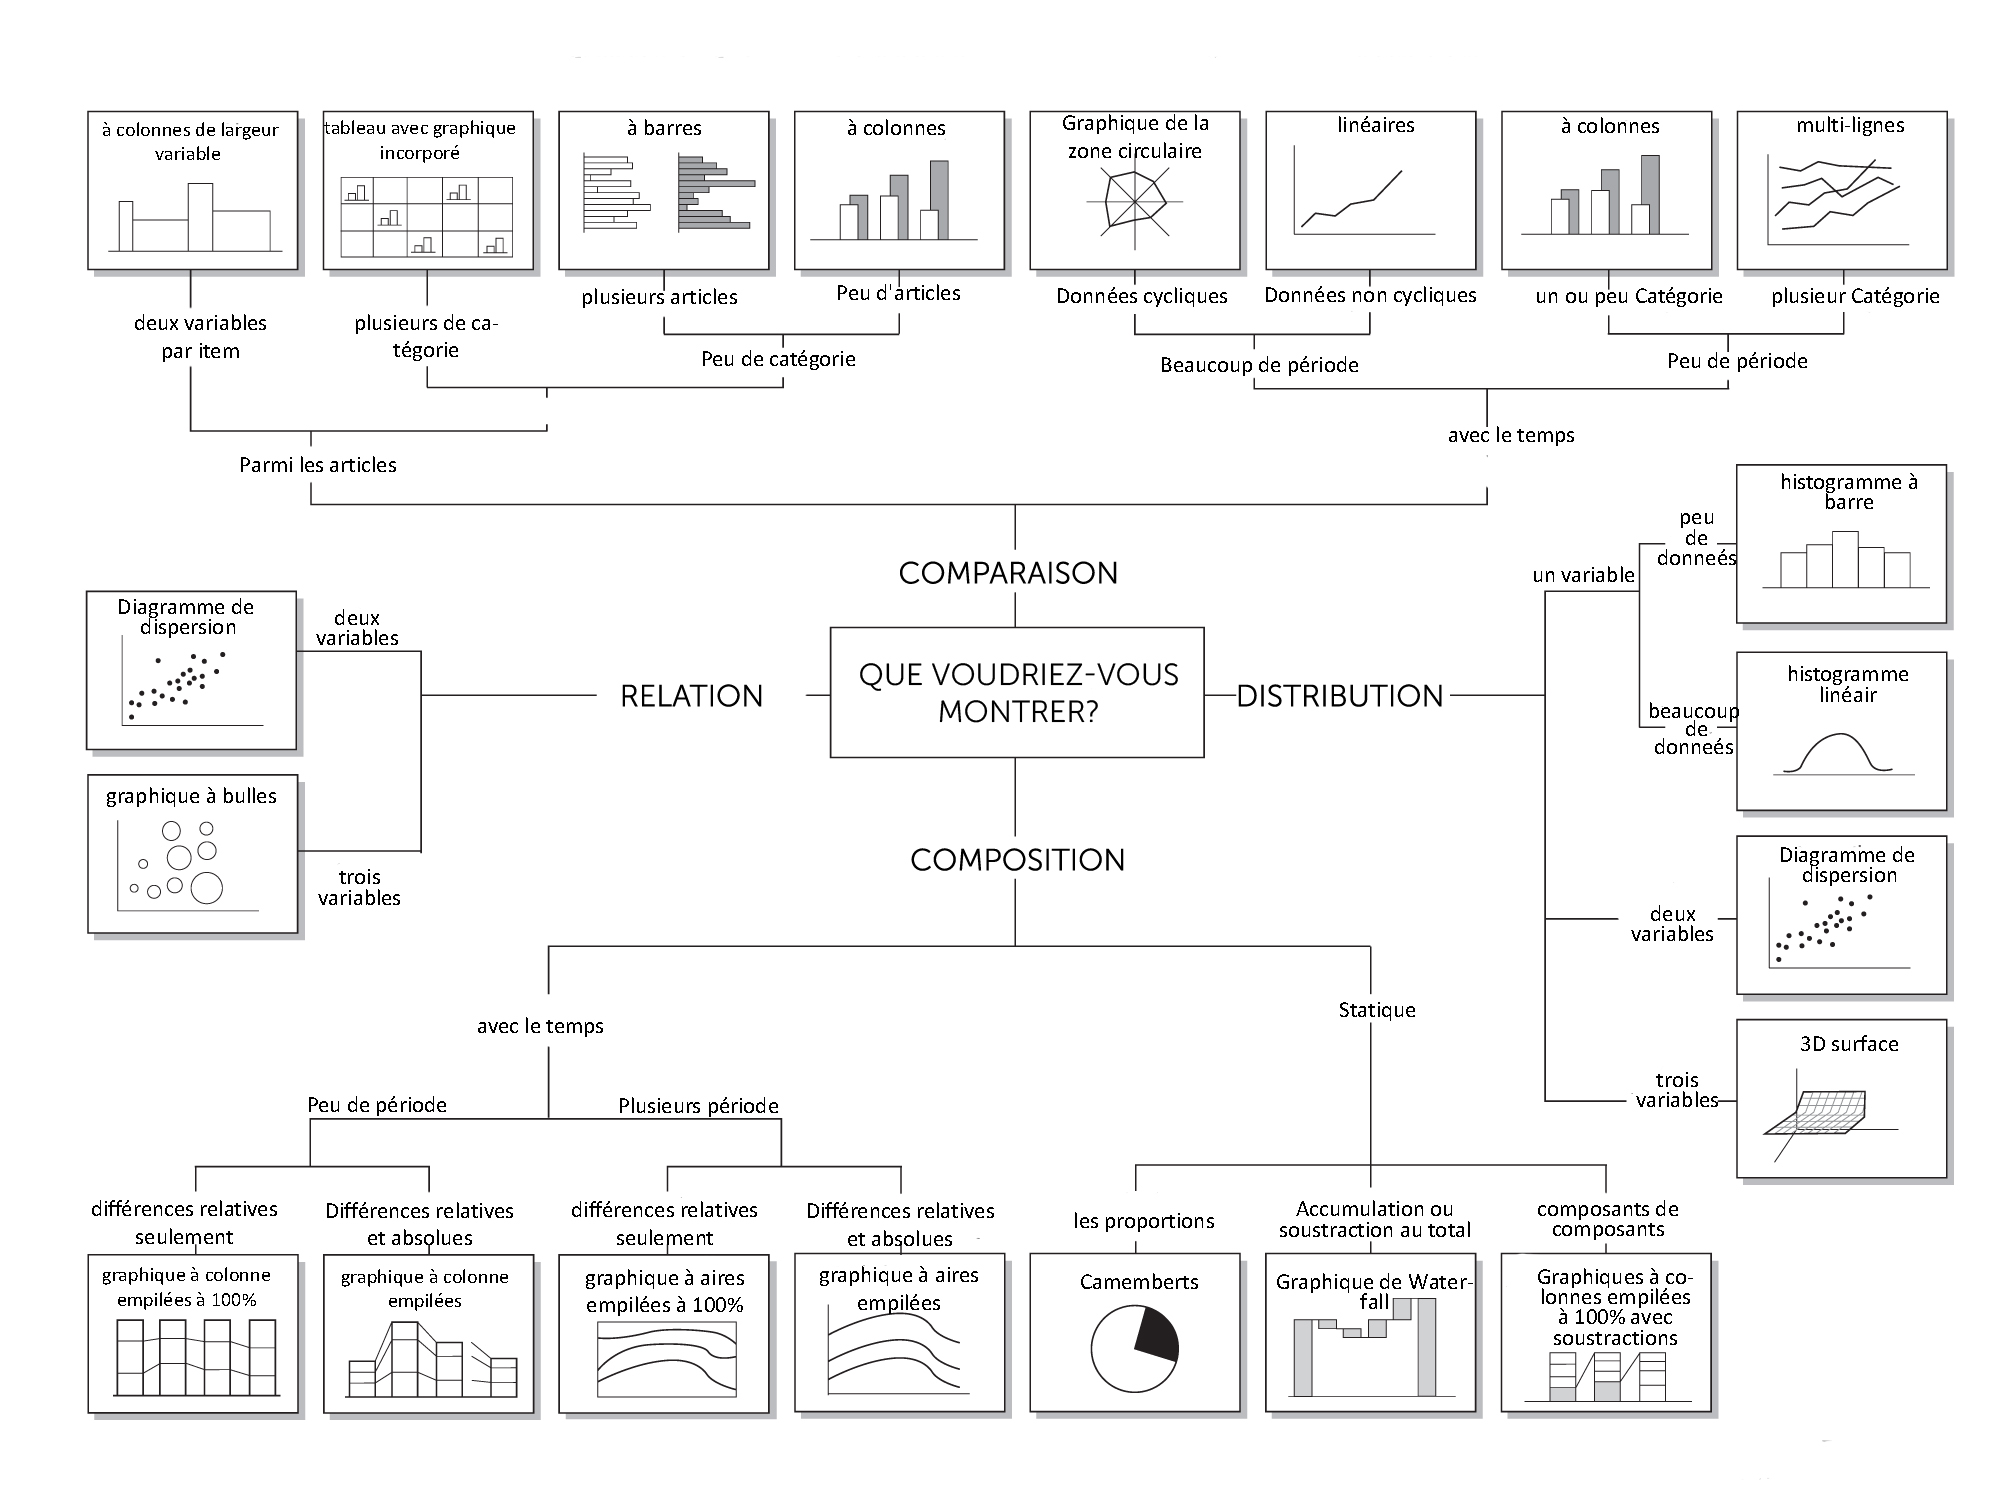
\includegraphics[height=8cm]{images/diagramme-de-charts.jpg}
    %\scriptsize{source:\url{add url}}
    \caption{Le diagramme de sélection de graphique}
    \label{fig:2.1}
\end{figure}
 Le diagramme de sélection de graphique illustré à la figure ~\ref{fig:2.1}
, permet de choisir le bon graphique en fonction du type de données.
\subsubsection{1. Comparaison: }
Ces visualisations se rapportent au temps et à la taille des données. Les graphiques de comparaison sont utilisés pour comparer la magnitude des valeurs et peuvent être utilisés pour trouver facilement les valeurs les plus basses et les plus hautes dans les données. Les graphiques de comparaison peuvent être également utiliser pour comparer les valeurs actuelles par rapport aux valeurs anciennes afin de déterminer si les valeurs augmentent ou diminuent. Les questions les plus courantes sont «quels produits se vendent le mieux» et «comment nos ventes se comparent-elles à celles de l'année dernière».
Il n’existe pas un seul graphique à utiliser pour toutes les données synchronisées; certaines situations requièrent des graphiques linéaires tandis que d'autres nécessitent des graphiques à barres ou des graphiques en aires (pour les données cycliques).
Par exemple, pour un nombre moins élevé de catégories parmi les éléments, le  graphique à barres affiche mieux les différences entre les données que les camemberts. C’est la raison pour laquelle il est préférable d’utiliser un graphique à barres qu’un graphique à secteurs lorsqu'il est question de comparaison.
\subsubsection{2. Composition:}
Les graphiques de composition sont utilisés pour voir comment une partie se compare à la totalité et comment une valeur totale peut être divisée en plusieurs valeurs. Un graphique de composition montre la valeur relative, mais certains graphiques peuvent également être utilisés pour montrer la différence absolue. La différence est entre regarder le pourcentage du total et la valeur du total. Les questions communes sont «quelle part du marché nous avons dans une région» ou «en quels domaines notre budget est-il divisé».
Ces visualisations font référence à des ensembles de données qui évoluent dans le temps ou incluent des données statiques. Avec les données statiques, un diagramme à secteurs peut fonctionner.
\subsubsection{3. Relations : }
Les diagrammes de relations sont utilisés pour voir la relation entre les données et peuvent être utilisés pour trouver des corrélations, des valeurs aberrantes et des grappes de données. Les questions courantes sont les suivantes: «existe-t-il une corrélation entre les dépenses publicitaires et les ventes de nos produits» ou «comment les dépenses et les revenus varient-ils d’une région à l’autre et quel est l’écart»

\subsubsection{4. Distribution: }
Les graphiques de distribution sont utilisés pour voir comment les valeurs quantitatives sont réparties le long d'un axe, du plus bas au plus élevé. En examinant la forme des données, un utilisateur peut identifier des caractéristiques telles que la plage de valeurs, la tendance centrale, la forme et les valeurs aberrantes. Il peut être utilisé pour répondre à des questions telles que «nombre de clients par groupe d'âge» ou «combien de jours en retard ont nos paiements».
Pour illustrer mieux ce type de graphique, le graphique de nuages de points (Scatter plot) est présenté ci-dessous :
\pagebreak

En affichant une variable dans chaque axe, il est possible de détecter une relation ou une corrélation entre les deux variables.
\begin{figure}[!htb]
\begin{minipage}{0.46\linewidth}
Différents types de corrélation peuvent être interprétés à travers les modèles affichés sur les diagrammes de dispersion. Il existe une corrélation positive (les valeurs augmentent ensemble), négative (une valeur diminue avec l’augmentation), nulle (pas de corrélation), linéaire, exponentiel et en forme de U. La force de la corrélation peut être déterminée par la proximité des points sur le graphique. Les points qui finissent loin du groupe général de points sont appelés points aberrants.
Des lignes ou des courbes sont ajustées dans le graphique pour faciliter l'analyse et sont dessinées aussi près que possible de tous les points. Ainsi, il est montré comment tous les points ont été condensés en une seule droite. Ceci est généralement connu sous le nom de Droite de meilleur ajustement et peut être utilisé pour effectuer des estimations par interpolation.
Les diagrammes de dispersion sont parfaits lorsqu’il est associé des données numériques et que l’objectif est de voir si une variable a un impact sur l'autre. Cependant, il est important de rappeler que la corrélation n'est pas une cause et qu'une autre variable inaperçue peut influer sur les résultats.
\end{minipage}\hfil
\begin{minipage}{0.35\linewidth}
    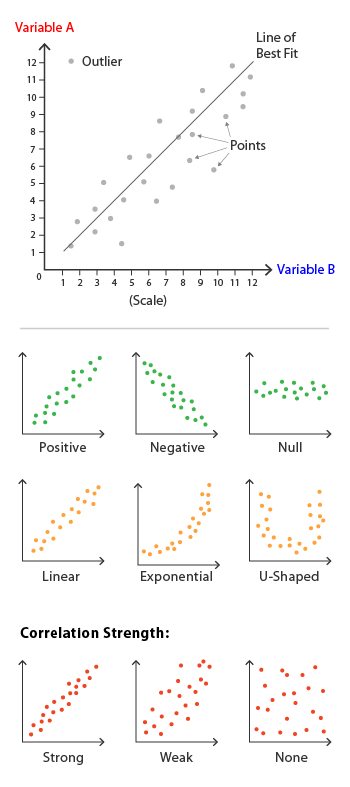
\includegraphics[height=13cm]{images/scatter-plot.png}
    \scriptsize{source :\url{https://datavizcatalogue.com/methods/scatterplot.html}}
    \caption{Diagramme de dispersion}
 \label{fig:1.6}
\end{minipage}
\end{figure}
\subsection{Infographie}
Les infographies sont devenues un moyen de communication de masse; ils sont conçus pour atteindre un public plus large en simplifiant les sujets complexes et en les organisant dans un format facile à digérer, contrairement à d'autres types de visualisations. \\*
Une infographie (graphique d'information) est une représentation visuelle de l'information qui vise à rendre les données facilement compréhensibles au premier coup d'œil. Une infographie utilise au minimum le texte et peut constituer un outil puissant pour afficher des données, expliquer des concepts, simplifier les présentations, cartographier les relations, afficher les tendances et fournir des informations essentielles.Les infographies se présentent sous différentes formes. Ils sont classés en fonction de leur objectif, des types d’objets utilisés et du flux d’informations. 
\newpage
\begin{figure}[!ht]
    \centering
    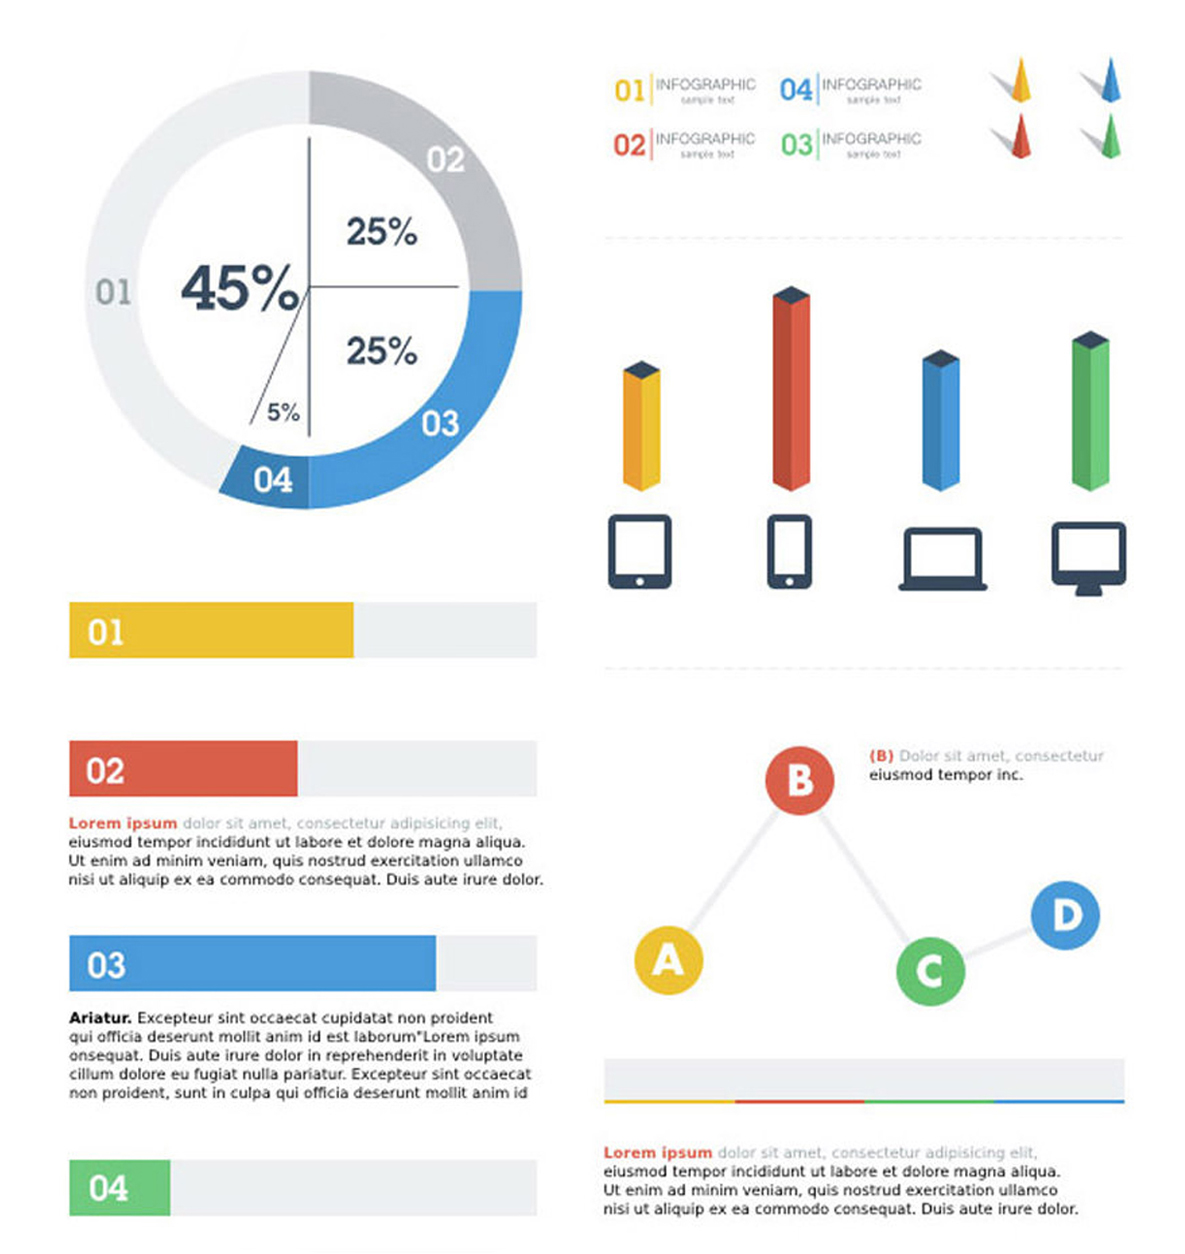
\includegraphics[height=10cm]{images/infographic.jpg}
    %\scriptsize{source:\url{add url}}
    \caption{infographic}
    \label{fig:2.1}
\end{figure}
\subsubsection{1. Infographie d'information}
L'infographie informationnelle se distingue par son utilisation de texte supérieure à la moyenne par rapport à d'autres types d'infographie. Le graphique peut être amélioré par des icônes, des formes, des couleurs et d'autres éléments visuels, mais dans l'ensemble, l'accent est mis sur les mots.

\subsubsection{2. Infographie de la chronologie }
L'infographie de la chronologie décrit les événements ou les actions dans un ordre chronologique. Ils sont souvent utilisés pour démontrer le développement d’un produit, une tendance historique ou l’évolution d’une idée. L'infographie de la chronologie utilise des icônes, des images et des éléments graphiques pour transmettre le message. Le format de la timeline peut être vertical, horizontal ou sinueux. Les infographies verticales et chronologiques sinueuses sont généralement plus faciles à lire. Une infographie de chronologie horizontale convient mieux aux affiches, aux présentations et aux environnements où l'espace n'est pas une contrainte.

\subsubsection{3. Infographie de graphiques }
L’infographie de graphiques a un graphique comme pièce maîtresse de la visualisation des informations. Des couleurs, des formes et des icônes peuvent être ajoutés à des fins d'emphase et/ou d'explication. Les graphiques fonctionnent mieux lorsqu’il est effectué une comparaison élémentaire d'éléments. 

\subsubsection{4. Infographie de graphiques en secteurs}
Les graphiques en secteur apparaissent assez souvent dans l'infographie, car ils sont très utiles quand il faut montrer des pourcentages d'un tout. Il est préférable d'utiliser les graphiques en secteur pour afficher des différences au sein d'un groupe en fonction d'une variable. Dans l'infographie, les graphiques en secteur viennent dans beaucoup de variantes et de styles pour montrer les différents composants d’un élément ou pour comparer une valeur à plusieurs autres valeurs.

\subsubsection{5. Infographie de processus }
L’infographie de processus décrit les processus de prise de décision. Les infographies de processus sont également appelées arbres de décision ou organigrammes. Chaque étape est liée à la suivante par des lignes et des flèches directionnelles. 

Alors qu'il existe différents types d'infographies, certains éléments sont essentiels pour rendre une représentation visuelle des données qualifiée d'infographie. Pratiquement toutes les infographies utilisent chacune d’elles dans une certaine mesure (couleurs, polices, icônes et images).

\subsection{Cartographie et Géomatique }
Le terme géomatique est un néologisme composé de « géo » (pour géographie) et de « matique » (pour informatique). C’est la discipline ayant pour objet « la gestion des données à référence spatiale et qui fait appel aux sciences et aux technologies reliées à leur acquisition, leur stockage, leur traitement et leur diffusion » (Marcel Bergeron, 1993, Vocabulaire de la Géomatique Québec). En somme, la géomatique est le domaine de l’informatique auquel se rattache les SIG (Système d’Information Géographique).
La cartographie incorpore trois dimensions sous-jacentes:

\begin{itemize}
\item \textbf{Une dimension informatique:}  aujourd’hui, sauf dans la volonté de produire une image originale à forte valeur artistique, plus personne ne réalise de carte à la main mais via des logiciels spécialisés. 
\item \textbf{Une dimension spatiale:}  l’information géographique (localisée dans l’espace) est la matière première du cartographe. 
\item \textbf{ Une dimension graphique:} cartographier, c’est dessiner l’espace géographique, ses continuités, ses ruptures. C’est mettre sur écran une représentation schématique de l’espace géographique.
\end{itemize} 
Le processus de conception cartographique concerne une transformation systématique des données spatiales en un affichage spatial multidimensionnel. Ce processus est généralement exécuté en appliquant des méthodes de «conception cartographique scientifique», ainsi que des règles esthétiques.

En cartographie, une carte peut fournir un aperçu général d’une zone géographique avec différents niveaux de détail; le niveau et la surface dépendent du point de vue et de la fonction du cartographe. Les cartographes utilisent plusieurs méthodes pour créer des cartes thématiques, mais quatre méthodes sont plus courantes:
\subsubsection{1. Les cartes à points (Dot Map)}
Les cartes à points sont un moyen de détecter les modèles spatiaux ou la distribution des données sur une région géographique, en plaçant des points de taille égale sur une région géographique.
Il existe deux types de cartes à points : un en un (un point représente un seul compte ou un objet) et un en plusieurs (un point représente une unité particulière, par exemple 1 point = 10 arbres).
Les cartes à points sont idéales pour voir comment les choses sont réparties sur une région géographique et peuvent révéler des motifs lorsque les points se regroupent sur la carte. Les cartes à points sont faciles à comprendre et donnent un meilleur aperçu des données, mais ne sont pas très utiles pour récupérer des valeurs exactes.
\begin{figure}[!ht]
    \centering
    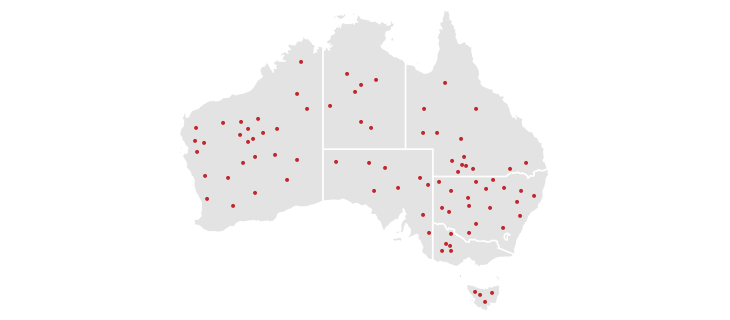
\includegraphics[height=5cm]{images/dot_map.png}
    \scriptsize{source :\url{https://datavizcatalogue.com/methods/dot_map.html}}
    \caption{Carte à point}
    \label{fig:1.7}
\end{figure}
\subsubsection{2. Les cartes à bulle (Bubble Map)}
Avec cette carte de données, les cercles sont affichés sur une région géographique désignée, la surface du cercle étant proportionnelle à sa valeur dans le jeu de données. Les cartes à bulles permettent de comparer des proportions sur des régions géographiques sans les problèmes causés par la taille de la région, comme le montre la carte de Choropleth. Cependant, l'un des principaux défauts de la carte à bulle est que des bulles trop volumineuses peuvent chevaucher d'autres bulles et régions sur la carte. Il faut donc en tenir compte.
\begin{figure}[!ht]
    \centering
    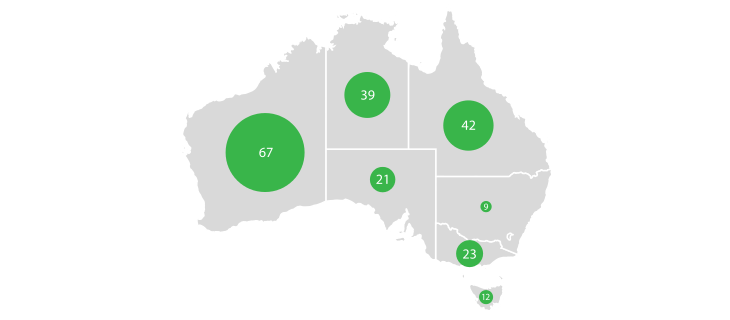
\includegraphics[height=5cm]{images/bubble_map.png}
    \scriptsize{source :\url{https://datavizcatalogue.com/methods/bubble_map.html}}
    \caption{Carte à bulle}
    \label{fig:1.8}
\end{figure}
\subsubsection{3. Les cartes Choroplèthes (Choropleth Map)}
Les cartes Choroplèthes affichent des zones géographiques ou des régions divisées colorées, ombrées ou structurées par rapport à une variable de données. Cela fournit un moyen de visualiser les valeurs sur une zone géographique, ce qui peut montrer des variations ou des modèles sur l'emplacement affiché.
La variable de données utilise la progression de la couleur pour se représenter dans chaque région de la carte. En règle générale, il peut s'agir d'un mélange d'une couleur à une autre, d'une progression de teinte unique, transparente à opaque, claire à sombre ou d'un spectre de couleurs complet.
\begin{figure}[!ht]
    \centering
    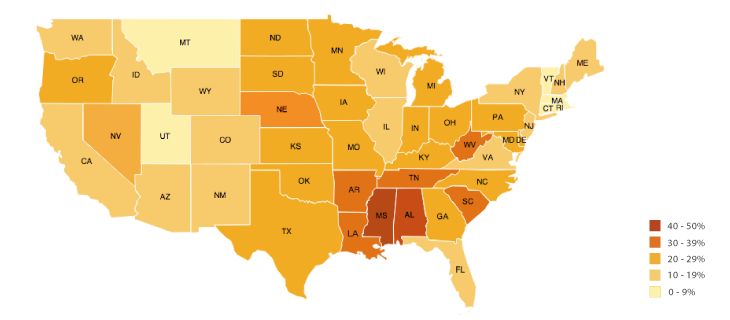
\includegraphics[height=5cm]{images/choropleth.png}
    \scriptsize{source :\url{https://datavizcatalogue.com/methods/choropleth.html}}
    \caption{Carte Choroplèthes 1}
    \label{fig:1.9}
\end{figure}

\begin{figure}[!htb]
\begin{minipage}{0.46\linewidth}
Un inconvénient de l'utilisation de la couleur est qu’il n’est pas possible de lire ou comparer avec précision les valeurs de la carte. Un autre problème est que les grandes régions apparaissent plus accentuées que les plus petites, ce qui affecte la perception des valeurs ombragées par l’utilisateur. 

Une erreur courante lors de la production de cartes Choroplèthes est de coder des valeurs de données brutes (telles que la population) plutôt que d'utiliser des valeurs normalisées (calcul de la population par kilomètre carré, par exemple) pour produire une carte de densité.
\end{minipage}\hfil
\begin{minipage}{0.35\linewidth}
    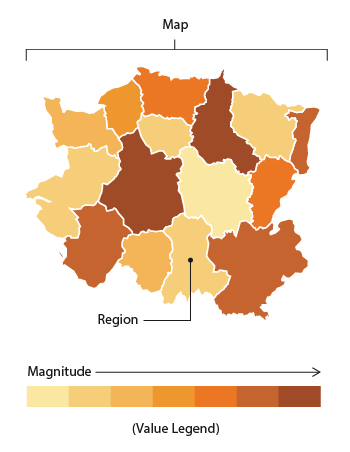
\includegraphics[height=8cm]{images/choropleth-zoom.png}
    \caption{Carte Choroplèthes 1}
 \label{fig:1.10}
\end{minipage}
\end{figure}
\subsubsection{4. Les cartes thermiques (Heatmap)}
La figure ~\ref{fig:1.11} ci-dessous montre les précipitations annuelles moyennes en Inde, en utilisant différentes nuances de bleu. Plus la nuance de bleu est sombre, plus les précipitations sont élevées.
\begin{wrapfigure}{R}{0.5\textwidth}
\centering
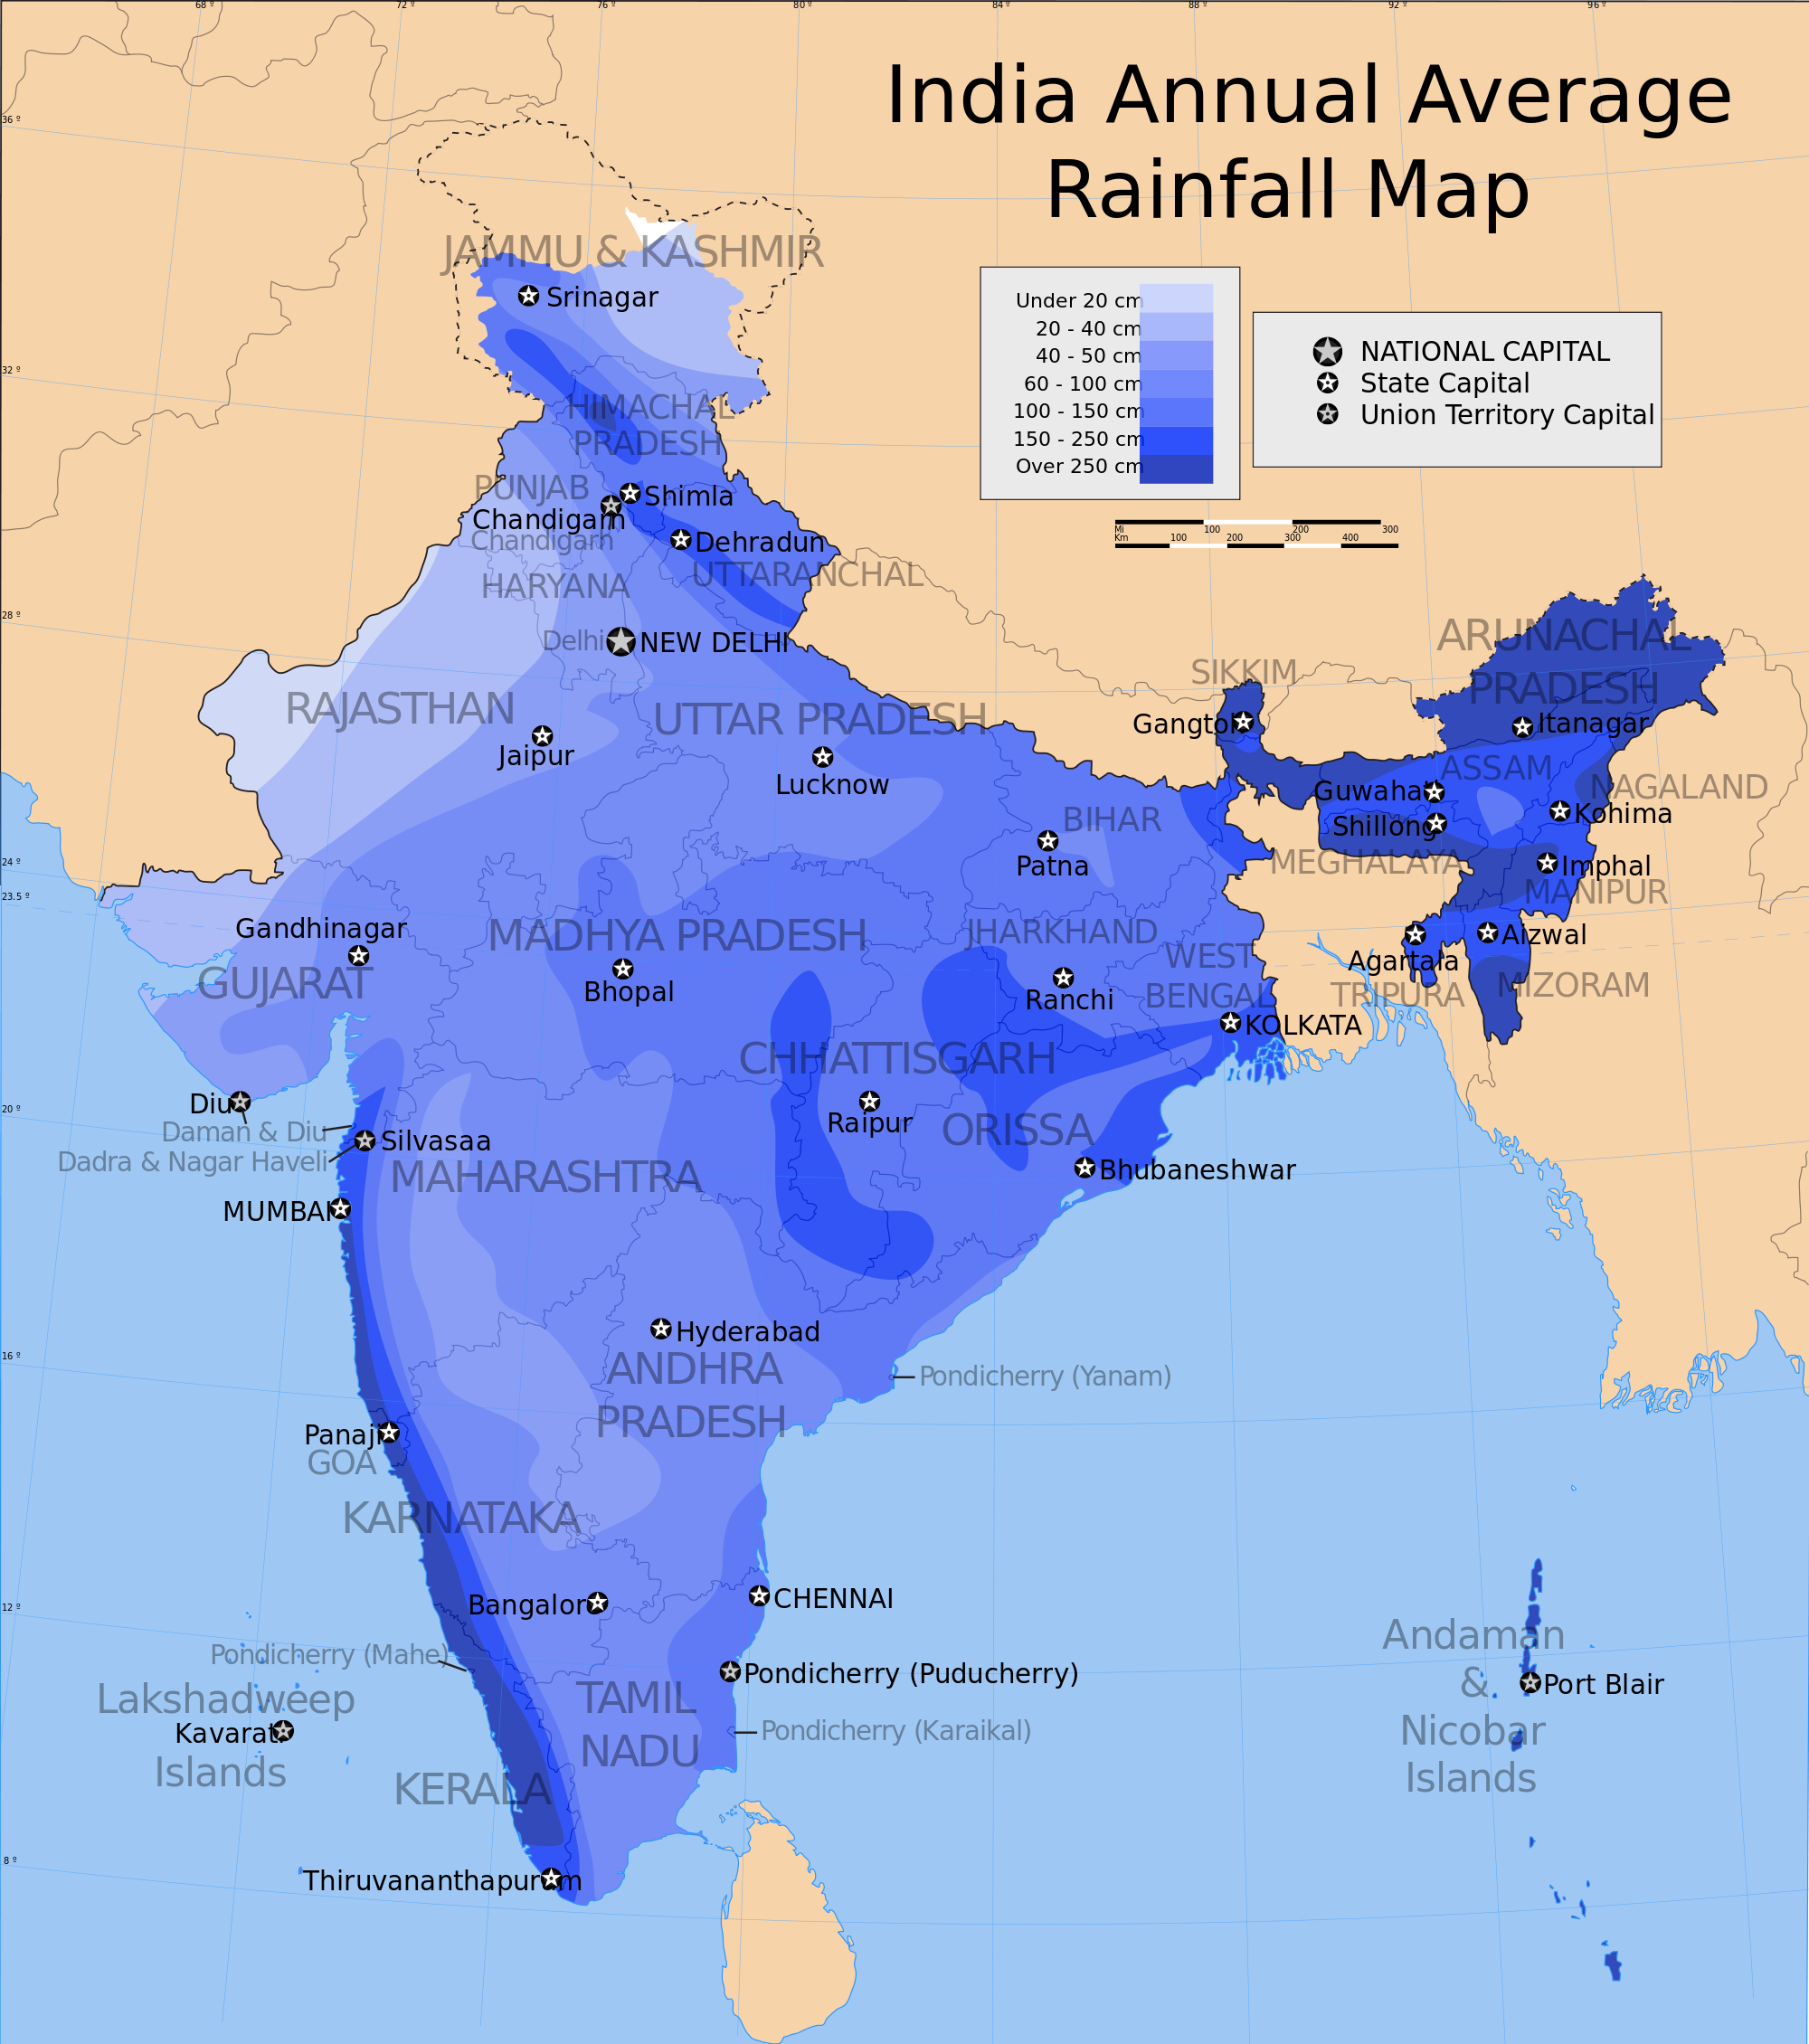
\includegraphics[width=0.4\textwidth]{images/Heatmap.png}
\scriptsize{source :\url{https://blog.socialcops.com/academy/resources/7-techniques-to-visualize-geospatial-data/}}
\caption{\label{fig:1.11} Carte thermique}
\end{wrapfigure}
Les cartes thermiques permettent de visualiser les données à travers des variations de coloration. Lorsqu'elles sont appliquées à un format tabulaire, les cartes thermiques sont utiles pour effectuer un examen croisé des données multivariées, en plaçant des variables dans les lignes et les colonnes, et en colorant les cellules du tableau. Les cartes thermiques sont utiles pour afficher la variance entre plusieurs variables, révéler toutes les tendances, indiquer si des variables sont similaires les unes aux autres et pour détecter si des corrélations existent entre elles. \\

En règle générale, toutes les lignes constituent une catégorie (étiquettes affichées à gauche ou à droite) et toutes les colonnes constituent une autre catégorie (étiquettes affichées en haut ou en bas). Les lignes et les colonnes individuelles sont divisées en sous-catégories, qui correspondent toutes les unes aux autres dans une matrice. Les cellules contenues dans le tableau contiennent des données catégoriques à code de couleurs ou des données numériques, basées sur une échelle de couleurs. Les données contenues dans une cellule sont basées sur la relation entre les deux variables de la ligne et de la colonne de connexion.

Une légende est nécessaire à côté d’une carte thermique pour que celle-ci puisse être lue avec succès. Les données catégorielles sont codées par couleur, tandis que les données numériques nécessitent une échelle de couleurs qui se mélange d'une couleur à l'autre afin de représenter la différence entre les valeurs hautes et basses. 
Les cartes thermiques peuvent également être utilisées pour afficher les modifications des données au fil du temps si l'une des lignes ou des colonnes est définie sur des intervalles de temps. Par exemple, utilisez une carte thermique pour comparer les changements de température au cours de l’année dans plusieurs villes, afin de déterminer les endroits les plus chauds ou les plus froids. Ainsi, les lignes pourraient répertorier les villes à comparer, les colonnes contiennent chaque mois et les cellules contiennent les valeurs de température.


\subsection{La Géovisualisation}
La géo-visualisation et l'analyse visuelle de données géospatiales sont devenues un centre d'intérêt pour la recherche, les industries, le gouvernement et d'autres organisations pour améliorer la mobilité, l'efficacité énergétique, la gestion des déchets et l'administration publique d'une ville intelligente.\\

La géovisualisation communique les informations géospatiales d'une manière qui, associée à la compréhension humaine, permet l'exploration des données et la prise de décisions. Les cartes statiques traditionnelles ont une capacité d'exploration limitée. La géovisualisation permet des cartes plus interactives, y compris la possibilité d'explorer différentes couches de la carte, d'effectuer un zoom avant ou arrière, de modifier l'aspect visuel de la carte et d’apporter des modifications à une carte en temps réel permettant aux utilisateurs d’ajuster les données cartographiées. La géovisualisation représente un ensemble de technologies et de pratiques cartographiques qui tirent parti de la capacité des technologies modernes. Il est important de rendre les données complexes plus claires et utiles grâce à une conception visuelle appropriée, par exemple en inventant de nouvelles métaphores visuelles, en créant des algorithmes d'analyse, etc. \\*
L'analyse visuelle intègre de nouveaux outils avec des techniques interactives innovantes et des représentations visuelles pour permettre une interaction homme-information. La conception des outils et des techniques repose sur des principes cognitifs et perceptuels. Cette science du raisonnement analytique fournit le cadre sur lequel il est possible de construire des technologies d'analyse visuelle stratégiques et tactiques pour l'analyse des menaces, la prévention et la réaction.
Les outils d'analyse visuelle doivent permettre différentes tâches d'analyse, telles que:

\begin{itemize}
\item Comprendre rapidement les situations, ainsi que les tendances et les événements qui ont généré les conditions actuelles.
\item Identifier les futurs possibles et leurs signes avant-coureurs
\item Surveiller les événements actuels pour détecter l'apparition de signes avant-coureurs et d'événements imprévus.\\
\end{itemize}

La gestion des données spatiales joue un rôle fondamental dans la conception de l’information urbaine. La conception de l'information urbaine est l'un des outils les plus importants dans l'analyse des processus urbains et dans la planification d'une «ville intelligente».

Ces dernières années, différentes techniques de représentation des données spatiales ont été considérablement développées dans différents types de cartes (cartes de points, de lignes, de polygones, de cartes choroplèthes, de cartes isoplèthes, de cartogrammes, etc).\\ Les indicateurs spatiaux peuvent être représentés de différentes manières: en deux ou en trois dimensions, en fonction du caractère bidimensionnel ou tridimensionnel des phénomènes. Si le phénomène analysé a principalement deux dimensions, il est courant de le représenter en utilisant le même nombre de variables spatiales. 
La représentation consiste à faire des choix qui nécessitent un premier niveau d’analyse pour extraire la signification et la transmettre à l’utilisateur via une représentation graphique, telle que la carte ou la visualisation 3D illustré ci-dessous. 


\begin{figure}[!ht]
    \centering
    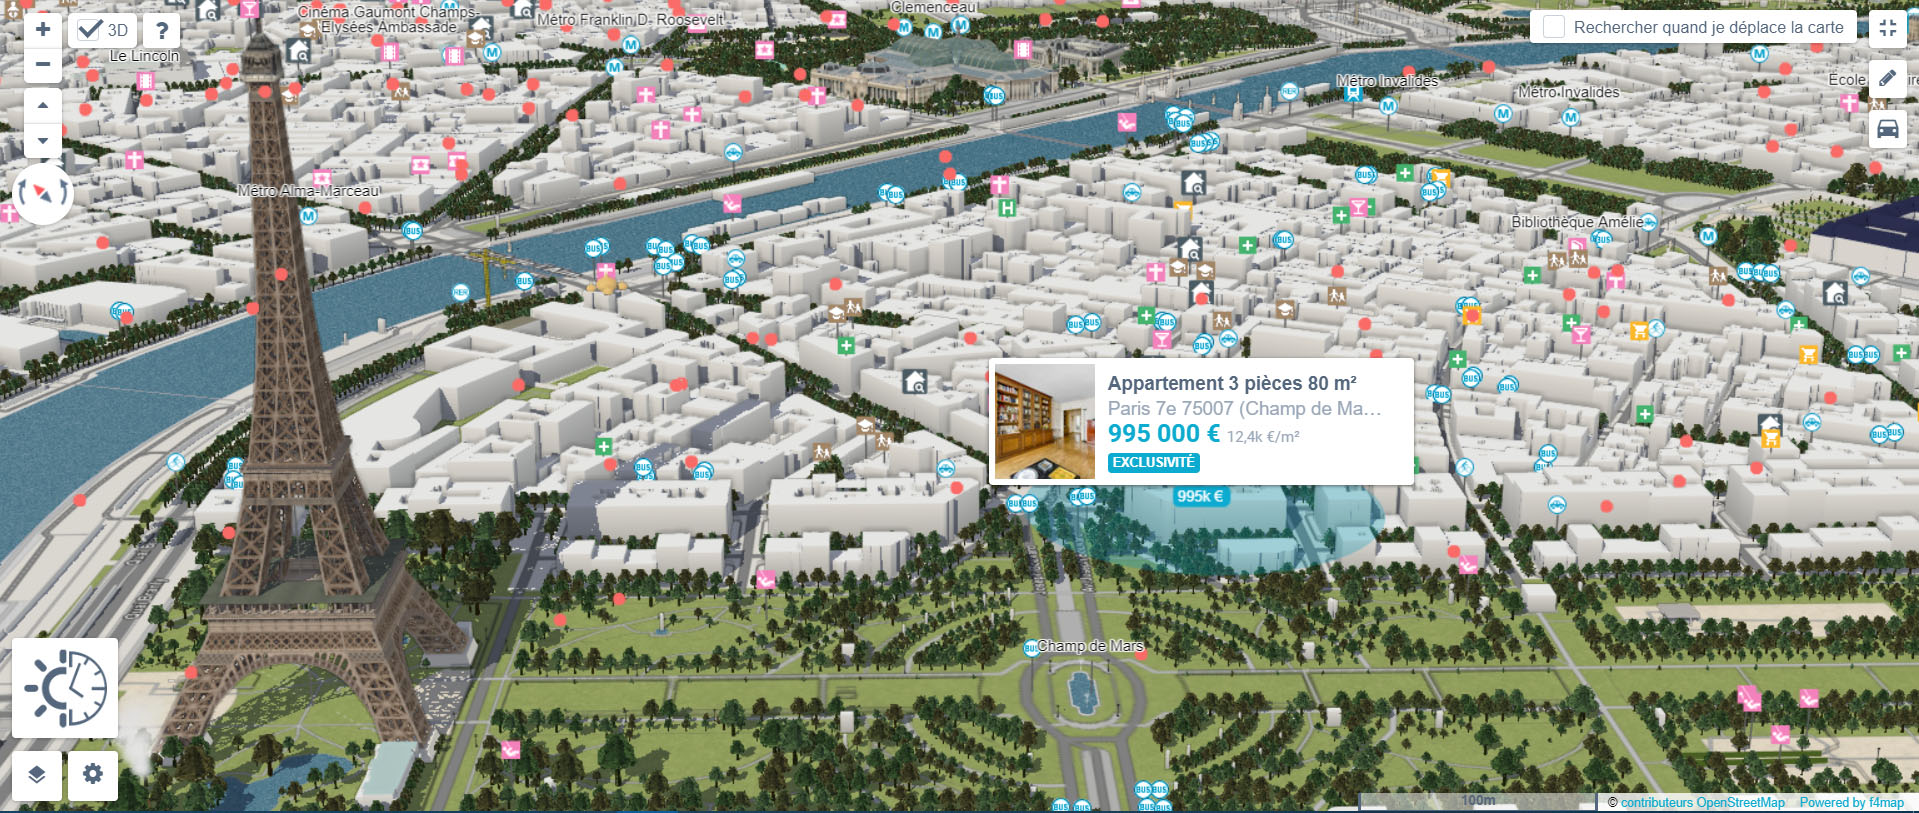
\includegraphics[height=6.6cm]{images/bienIci.jpg}
    %\scriptsize{source :\url{https:// }}
    \caption{capture d'écran du site Bien’Ici }
    \label{fig:2.9}
\end{figure}
La figure ~\ref{fig:2.9} présente une nouvelle approche pour la recherche immobilière, plus simple, plus rapide et plus agréable pour les internautes par l’entreprise Bien’Ici . Sa cartographie en 3D était développée par l’agence de jeux vidéos F4Map\footnote{ La carte F4 (F4Map) est une carte 3D basée sur Openstreetmap qui utilise la technologie WebGL } qui a modélisé la France entière en 3D. La carte passe automatiquement en 3D à partir d’un certain niveau de zoom. Toutes les annonces sont repérables sur la carte par un point rouge ou une étiquette de prix.  La carte en 3D permet de déplacer dans tous les sens afin de découvrir le logement et le quartier sous tous les angles.

%%%%%%%%%%%%%%%%%%%%%%%%%%%%%%%%%%%%%%%%%%%%%%%%%%%%%%%%%%%%%%%%%%%%%
\section{Outils de visualisation du Big Data: }
Les outils de visualisation de données sont exactement les armes dont nous avons besoin. Ces outils nous montrent diverses informations sur les données collectées. Les grands entreprises tels que Google et Microsoft collectent et manipulent des données volumineuses pour concevoir l'avenir de leurs stratégies commerciales. Cette section couvre certains outils de visualisation associés au Big Data. Les outils de visualisation sont diverses.  Plusieurs approches se sont dégagés selon le contexte. \\

\subsection{Approche de visualisation de JS}
Cette approche contient l’ensemble des bibliothèques de Java Script spécialisées dans la visualisation de données. Elle aide les développeurs qui confectionnent des applications web ou mobile à visualiser les données dans leurs propres applications. 
Parmis les nombreuses bibliothèques Javascript, les six bibliothèques les plus utilisées sont décrites ci-dessous : 
\subsubsection{1. Data Driven Document «D3.js»}
D3.js est une bibliothèque Javascript permettant de visualiser le Big Data de la manière que le développeur souhaite. Une connaissance solide en Javascript du développeur est nécessaire pour donner une forme aux données collectées. 

D3.js est très complète avec beaucoup d’exemples à disposition, avec une personnalisation totale possible. Elle permet l’accès à des primitives SVG permettant toute innovation. Les données peuvent être sous différents formats, le plus souvent JSON,  CSV ou geoJSON. Ces principales caractéristiques sont : 

\begin{itemize}
    \item Prise en charge de nombreux types de graphiques, bien plus que la grande majorité des autres bibliothèques de graphiques JavaScript.
    \item Combine des composants de visualisation puissants et une approche de manipulation DOM basée sur les données.
    \item Facile à déboguer à l'aide de l'inspecteur d'éléments intégré au navigateur.
    \item Des centaines d'exemples.
    \item Glisser déposer , zommer et d'autre.
    \item D3 est une bibliothèque JavaScript open source pour les graphiques, qui est gratuite pour tout type d'utilisation.
    
\end{itemize}
\subsubsection{2. Chartist.js}
Chartist.js est une bibliothèque JS open source non intrusive qui peut également être utilisée pour créer des graphiques réactifs. Chartist convient aux utilisateurs qui ont besoin d’un graphique très simple (lignes, barres ou secteurs) et qui n’exigent pas beaucoup de visualisation de données. Les principales caractéristiques sont :
\begin{itemize}
\item \textbf{} Nombre de types de graphiques restreint
\item \textbf{} Possibilité d’ajouter des animations.
\item \textbf{} La documentation de l’API contient toutes les informations
\item \textbf{}  Nécessaires, mais peu pratique à utiliser et nécessitant de longs parchemins.
\item \textbf{} Permet d'utiliser des plugins pour étendre les fonctionnalités.
\item \textbf{} Utilise SVG pour dessiner les graphiques (compatibles à l’avenir).
Vieux navigateurs supportés.
\item \textbf{} Open source, gratuit pour tout type d’utilisation.
\end{itemize} 
\subsubsection{3. Chart.js}
Chart.js est une bibliothèque JavaScript simple et flexible pour la visualisation de données. C’est une excellente solution de base pour les développeurs qui ne nécessitent pas de nombreux types de graphiques et de fonctions de personnalisation, mais qui souhaitent que leurs graphiques soient nets, clairs et instructifs. Les principales caractéristiques sont : 
\begin{itemize}
\item \textbf{} Huit types de graphique: ligne, zone, barre, camembert, radar, polaire, bulle et diffusion.
\item \textbf{} Tous les types de graphique peuvent être personnalisés et animés.
\item \textbf{}  Lorsqu'ils sont utilisés en ligne, tous les graphiques sont réactifs.
\item \textbf{} La fonctionnalité peut être étendue grâce à l'utilisation de plugins.
\item \textbf{} Une documentation assez riche.
\item \textbf{} Support via Stack Overflow.
\item \textbf{} Les navigateurs supportent IE9 +.
\item \textbf{} Une bibliothèque de graphiques JS open-source gratuite. Publié sous licence MIT.
\end{itemize} 
\subsubsection{4. HighCharts}
Highcharts est l’une des bibliothèques de graphiques JavaScript les plus complètes et les plus populaires, basée sur HTML5, avec un rendu au format SVG / VML. Il est léger, prend en charge un large éventail de types de graphiques et garantit des performances élevées. Les principales caractéristiques sont : 
\begin{itemize}
\item \textbf{} Une utilisation du JavaScript pur. 
\item \textbf{} Les données peuvent être chargées en externe.
\item \textbf{} Une documentation robuste, une référence API et une présentation de la communauté.
\item \textbf{} Une exploration des données du graphique et d'autres options d'interactivité.
\item \textbf{} Une utilisation possible avec différentes framework front-end tels que React, Angular, Meteor, .NET, iOS, etc.
\item \textbf{} Une exportation au format PNG, JPG, PDF ou SVG.
\item \textbf{} Gratuit pour les organismes à but non lucratif. Payé pour un usage commercial (à partir de 50 \$).
\end{itemize} 

\subsubsection{5. C3.js}

C3.js est une autre bibliothèque de diagrammes réutilisable. C3.js est Open Source et est basé sur la bibliothèque D3.js qui est actuellement très complète et permet de réaliser une grande diversité de rapports. Les principales caractéristiques sont :
\begin{itemize}
\item \textbf{} Grand nombre d’outils de cartographie basés sur D3.
\item \textbf{} Les graphiques sont interactifs et peuvent être dynamiques (onclick, onmouseover, etc). 
\item \textbf{} Il est également possible de les imprimer en PDF.
\item \textbf{} Pouvoir activer ou désactiver le zoom sur un graphique, charger des données depuis une url ou un fichier de type CSV, inverser les abscisses et ordonnées, modifier la « tooltip ».
\item \textbf{} Il fournit un certain nombre d'API et de callbacks pour mettre à jour le graphique.
\item \textbf{} Une bibliothèque de graphiques JS open-source gratuite. Publié sous licence MIT.
\end{itemize} 

\subsubsection{6. Plotly.js}
Plotly.js est une bibliothèque JavaScript de haut niveau, gratuite et à code source ouvert. Il est basé sur D3.js et WebGL. Il peut donc être utilisé pour créer de nombreux types de graphiques, notamment des graphiques 3D aux graphiques statistiques. Les principales caractéristiques sont : 
\begin{itemize}
\item \textbf{} 20 types de graphiques pouvant être intégrés à des sites Web ou utilisés pour créer des présentations dynamiques.
\item \textbf{} Utilisée comme une bibliothèque de graphiques basée sur un navigateur pour Python, R et MATLAB, en résumant des graphiques en une structure JSON déclarative.
\item \textbf{} Permet d'utiliser des feuilles de calcul Excel ou de se connecter à votre base de données.
\item \textbf{} Exportation de graphiques en PNG et JPG; EPS, SVG et PDF sont disponibles sur abonnement.
\item \textbf{} Documentation complète sur les API.
\item \textbf{} Open-source, bibliothèque gratuite.
\end{itemize} 
\subsubsection{7. Nvd3}
NVD3 est une bibliothèque Javascript visant à créer des graphiques et des composants réutilisables pour D3.js, en offrant les mêmes fonctionnalités puissantes, mais beaucoup plus simple à utiliser. Elle permet de gérer des ensembles de données complexes et de créer des visualisations avancées.

\subsection{Approche de visualisation des BI}
Les outils d'aide à la décision ont pour objectif d’aider à comprendre les tendances et à tirer parti de données pour permettre de prendre des décisions commerciales stratégiques.
Ces outils permettent de réaliser des graphiques, des présentations et des tableaux de bord en toute simplicité. Les analyses de données peuvent être effectuées à l’aide de JavaScript, Python, R, Matlab, Jupyter ou encore Excel. 
Cependant, avec le nombre important d’outils de BI sur le marché, le démarrage du processus de sélection peut être difficile. Parmi ceux-ci , les trois BI les plus utilisés selon les statistiques sont : 
\subsubsection{1. Sisense}
Le logiciel de BI Sisense permet aux entreprises de rassembler, d’analyser et de visualiser des données pouvant être utilisées pour prendre de bonnes décisions et d’élaborer des plans stratégiques. L'outil regroupe toutes les informations nécessaires dans un tableau de bord unique avec sa fonctionnalité de glisser-déposer et fournit une vue granulaire des données. Les utilisateurs peuvent proposer une analyse fiable en utilisant des rapports visuels comme base, ce qui simplifie considérablement le processus. L’interface de la plate-forme est facile à utiliser, permettant aux utilisateurs d’apprendre rapidement et facilement la navigation dans les systèmes. Les principaux avantages sont :
\begin{itemize}
\item \textbf{Utilisation rationnelle des ressources:}  la technologie In-Chip de Sisense optimise les ressources déjà existantes sur une machine en déterminant la meilleure utilisation possible de sa capacité pour stocker, compresser et accéder à plus de données plus rapidement. Sisense est capable de déplacer des données 50 à 100 fois plus rapidement que les solutions en mémoire en utilisant la mémoire disponible dans la CPU.
\item \textbf{Performances:}  Sisense est conçu avec une base de données en colonnes évolutive et optimisée en mémoire, capable de gérer des téraoctets de données et des dizaines de requêtes simultanées. Cela permet aux non-techniciens de joindre facilement des données provenant de sources multiples et de créer des visualisations et des rapports interactifs.
\item \textbf{ Réponse plus rapide:} le produit utilise la technologie BI d'accélération pour scinder chaque requête en blocs de requête et chaque bloc de requête est mis en cache individuellement. Cela se traduit par une réponse plus rapide aux nouvelles requêtes et permet au cache de rester efficace même lorsque le nombre d'utilisateurs et de requêtes augmente.
Consolidation de graphiq
\item \textbf{ues provenant de sources multiples:}  le pouvoir unique de Sisense est qu’il reconnaît et rassemble automatiquement des graphiques et des tableaux de différentes sources de données, puis combine les données qu’ils contiennent sans les préparer.
\end{itemize} 
\subsubsection{2. Tableau}
 Tableau aide les entreprises à visualiser et à comprendre les données. Il permet aux organisations de connecter, visualiser et partager des données via un PC ou un iPad. Les utilisateurs peuvent facilement créer des tableaux de bord, les publier et même les partager avec leurs collègues, partenaires et clients sans avoir besoin de connaissances en programmation. \\
 Le logiciel peut se connecter à de nombreuses sources d’information et importer et visualiser des informations dans un délai très court. Le logiciel est intuitif, facilitant l’utilisation et permettant l’analyse de données à l’aide de la fonctionnalité glisser-déposer. Il favorise la collaboration en permettant l’analyse de groupe et en informant tous les membres de l’équipe à tout moment. Les utilisateurs peuvent également accomplir des tâches pratiquement n'importe où et à tout moment, grâce à l'application mobile native.  Les principaux avantages sont :
 \begin{itemize}
\item \textbf{Glisser-déposer :} Tableau a été l'un des premiers systèmes de BI à présenter des tableaux de bord analytiques intuitifs dans lesquels les utilisateurs peuvent manipuler des données avec un simple mécanisme de glisser-déposer.
\item \textbf{Interactions de tableau de bord à tableau de bord :}  avec Tableau, il est possible de copier différents éléments de tableau de bord et les transférer dans d'autres classeurs. 
\item \textbf{Authentication SAML\footnote{Security assertion markup language (SAML) est un standard informatique définissant un protocole pour échanger des informations liées à la sécurité. Basé sur le langage XML, SAML a été développé par OASIS.} :} il s’agit d’une méthode open source permettant de créer une expérience de connexion unique. Ceci permet à Tableau de se connecter à n’importe quelle application / système tierce.
\item \textbf{Création avec Web mobile:}  Tableau affichera non seulement les données sur les appareils mobiles, mais il permettra également de modifier les vues existantes, d'analyser les données et d'enregistrer les nouvelles versions avec une application dédiée.
\end{itemize} 
\subsubsection{1. Power BI}
Microsoft Azure Power BI est un logiciel développé et prise en charge par Microsoft pour les besoins en matière de veille stratégique et d'analyse. Au cœur de Power BI se trouve un service en ligne offrant diverses options d’interaction, ainsi que plusieurs accès permettant la connexion aux données fournies.
Les principaux avantages sont :
\begin{itemize}
\item \textbf{Personnalisation riche des tableaux de bord :}  MS Power BI offre une expérience utilisateur unifiée avec des tableaux de bord et des rapports personnalisés qui répondent aux besoins exacts de l'utilisateur. 
\item \textbf{Géo-cartes :} Les visualisations de géo-cartes interactives sont également renforcées par Bing Maps.
\item \textbf{Publication sécurisée de rapports:}  la configuration de l'actualisation des données est automatique et la publication des rapports est rapide, permettant ainsi à tous les utilisateurs de bénéficier des dernières informations.
\item \textbf{Pas de contraintes de mémoire et de vitesse:} Pas de contraintes de mémoire et de vitesse: la récupération et l’analyse des données est rapide, en éliminant les contraintes de mémoire et de vitesse.
\item \textbf{Aucune assistance technique spécialisée n’est requise:}  l’utilisateur peut tirer parti des avantages des enquêtes et les analyses agiles sont offertes par Power BI, en éliminant ainsi le besoin d’une assistance technique spécialisée.
\item \textbf{La fonction de questions / réponses (Q & R):} il est constitue un avantage pour réaliser une BI en libre service.
\item \textbf{Innovation constante:}  le produit Power BI est mis à jour presque tous les mois avec de nouvelles fonctionnalités.\\
\end{itemize} 
Au total, il existe plus de 20 solutions BI sur le marché. Trois outils présentés ci-dessus font partis des solutions leaders. Il est très difficile aujourd’hui de faire un comparatif de tous ces produits. Cependant, ces solutions peuvent être classées sous deux catégories.
\begin{itemize}
\item \textbf{} Les solution BI intégrées, tels que Oracle Business Intelligence Foundation Suite, SAP BusinessObjects et IBM Cognos qui sont les leaders en matière d’ERP et qui intègrent leur couche BI dans leur produit pour la génération des rapports prédéfinis. Ces solutions sont plutôt adaptées aux grandes entreprises.
\item \textbf{} Les solutions d’exploration des données, tels que les produits dédiés à l’informatique décisionnelle et les outils offrant une fonction BI en self-service comme la suite SQL de microsoft, Qlik, Tableau, Tibco, Microstratégy, etc. 

\end{itemize} 

\subsection{Approche de visualisation de SIG}
La visualisation de données par la cartographie est devenue un moyen essentiel pour les villes intelligentes de tirer parti des données recueillies à partir de diverses technologies ou d’applications intelligentes. Les cartes de système d'information géographique (SIG) fournissent des éléments visuels faciles à assimiler qui peuvent aider les villes à déterminer les zones nécessitant certains aménagements ou services, ainsi que les meilleurs plans de répartition des ressources.
Parallèlement à l'explosion de l'analyse des données municipales, les outils de cartographie font leur apparition. Certaines d'entre elles sont destinées à des analyses de niche, d'autres à des analyses plus étendues, telles que les réparations nécessaires dans une ville. Bon nombre de ces applications vont au-delà du traçage des données existantes et fournissent également une analyse prédictive pour aider à prévenir et à résoudre les problèmes futurs des villes.
\subsubsection{1. ArcGIS}

ArcGIS est un système d'information géographique (SIG) permettant de travailler avec des cartes et des informations géographiques. Il est utilisé pour créer, manipuler des cartes, compiler des données géographiques, analyser des informations cartographiées, partager et découvrir des informations géographiques dans diverses applications et gérer des informations géographiques dans une base de données.








\subsubsection{2. QGIS}

Quantum GIS (QGIS) est un système d’information géographique (SIG) à source ouverte qui met en œuvre un grand nombre de fonctions d’accès, de visualisation, de traitement et d’analyse de données géospatiales. Il peut accéder aux données vectorielles stockées dans une grande variété de formats, y compris les fichiers (par exemple, fichiers de forme ESRI, KML, GML), les géodatabases (par exemple, PostgreSQL / PostGIs, ODBC, GéoDatabase personnelle ESRI, SQLite) et les protocoles réseau (OPeNDAP, GeoJSON); données raster dans l'un des 40 formats pris en charge par la bibliothèque raster GDAL sous-jacente (y compris NetCDF, HDF5, GeoTIFF, GRIB et JPEG-2000); et services de visualisation et d'accès aux données de Open Geospatial Consortium (services de cartographie Web et d'entités Web [WMS et WFS, respectivement]). Selon la configuration du système hôte, QGIS peut également servir d’interface utilisateur graphique alternative pour le grand nombre de fonctions de traitement géospatial GRASS GIS. QGIS comprend une architecture "plug-in" dans laquelle des extensions aux fonctionnalités principales de l'application peuvent être développées et utilisées, avec les plug-ins actuels, notamment la prise en charge de l'intégration GPS, l'interaction avec les serveurs de données OpenStreetMap et les outils de transformation de données.


\section{Etude comparative sur les approches }
















%%%%%%%%%%%%%%%%%%%%%%%%%%%%%%%%%%%%%%%%%%%%%%%%%%%%%%%%%%%%%%%%%%%
\chapter{ Etude comparative sur les outils de SIG }

\chapter{Cas pratique: visualisation du Big Data chez Datategy}
\section{Presentation de Datategy}
DATATEGY est une société de conseil et d’expertise en Data Science. Elle conçoit, développe et commercialise une plateforme prédictive de lutte contre la fraude basée sur les technologies d’intelligence artificielle 100\% cloud......
\section{Presentation d’OctoCity solution}
La Smart City, ou ville intelligente consiste globalement en l’optimisation des coûts, de l’organisation, du bien-être des habitants.La ville est au service du citoyen mais ce dernier a néanmoins des obligations à respecter pour s’inscrire lui même comme acteur bénéficiant de ses services .Nous agissons en droite ligne avec l’objectif des opérateurs, des métropoles, et des territoires afin d’accompagner cet enjeu sociétal, politique et environnemental.Les solutions développées par DATATEGY s’interconnectent avec les réseaux existants, le croisement et l’exploitation des données.......
\section{Etude comparative entre les différent bibliothèque de la visualisation}
L'objectif de cette partie est de présenter les tâches qui été réalisés sur la visualisation de Big data dans le cadre de la solution OctoCity.(état de l’art- Critiques - proposition et réflexion).

%\subsubsection{blabla}
%\begin{figure}[!htp]
%    \centering
%    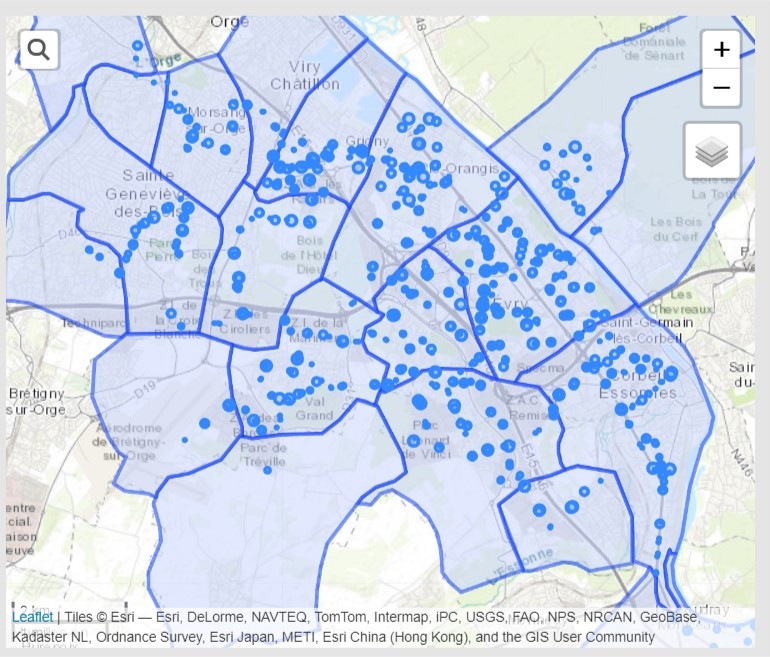
\includegraphics[height=6cm]{images/datategy-bubble-map.jpg}
%    \scriptsize{}
%    \caption{Visualisation le numbre de controle}
%    \label{fig:3.1}
%\end{figure}



\chapter{ Bilan et conclusion}
\section{Bilan professionnel}
\section{Bilan personnel}
\section{Conclusion}
En conclusion ...... 

% \nocite{*}
% \bibliographystyle{plain}
% \bibliography{biblio} 
% \phantomsection 
\addcontentsline{toc}{chapter}{Bibliographie} 
\begin{thebibliography}{9}
\bibitem{0}
United Nations. \emph{P.D.: The World’s Cities in 2016. United Nations}. [2016].

\bibitem{1} Neirotti \emph{, P., De Marco, A., Cagliano, A.C., Mangano, G., Scorrano, F.: Current trends in Smart City initiatives: some stylised facts. Cities 38, 25–36}. [2014]


\bibitem{2}  Liotine, M., Ramaprasad, \emph{, A., Syn, T.: Managing a Smart City’s resilience to Ebola: an ontological framework. In: 2016 49th Hawaii International Conference on System Sciences (HICSS), pp. 2935–2943. IEEE (2016)}. [2016]

\bibitem{3} Nam, T., Pardo\emph{, T.A.: Conceptualizing smart city with dimensions of technology, people, and institutions. In: Proceedings of the 12th Annual International Digital Government Research Conference: Digital Government Innovation in Challenging Times, pp. 282–291. ACM}.

\bibitem{4}IESE\emph{Ranking The World’s ‘Smartest’ Cities. Forbes. Forbes}. [2016]

\bibitem{5}Cameron, J.D., Ramaprasad, A., Syn,\emph{T.: An ontology of mHealth. Int. J. Med. Inform. 16–25}. [2017]

\bibitem{6} Murgante, B., Borruso,\emph{G.: Cities and smartness: the true challenge. Int. J. Agric. Environ. Inf. Syst. 6, 5}. [2015]

\bibitem{7}Khan Z, Anjum A, Kiani,\emph{SL. Cloud Based Big Data Analytics for Smart Future Cities. In Proceedings of the 2013 IEEE/ACM 6th International Conference on Utility and Cloud Computing. IEEE Computer Society; 2013. pp. 381–386.}

\bibitem{8} Rosa Marina Donolo,\emph{G.: Contributions to geovisualization for territorial
intelligence}. [2017]

\bibitem{11} Google Charts, Google \url{https://developers.google.com/chart/}. [2017]

\bibitem{12} Tableau,\url{https://public.tableau.com/s/}. [2003]

\end{thebibliography}
\end{document}
